\chapter{Additional Research}
\label{sec:additional}

\ifpdf
    \graphicspath{{8_additional/figures/PNG/}{8_additional/figures/PDF/}{8_additional/figures/}}
\else
    \graphicspath{{8_additional/figures/EPS/}{8_additional/figures/}}
\fi

The 3D mesh-based classification pipeline was considered successful in learning to differentiate between event and noise timeslices. However, feature engineering was required to be able to learn sufficiently (Appendix \ref{appendix}). Qi et al. (2017) had highlighted that PointNet could work with just 3D coordinates \cite{qi2017pointnet}. Therefore, additional research was conducted to explore an alternate 3D point-based pipeline. If successful, it would simplify the computational costs and research time. The 3D point-based pipeline was next expanded to a 4D PointNet. Instead of generating three datasets out of  \texttt{x, y, z} and \texttt{time}, they could be directly used as 4D points to train PointNet. The final section of this chapter provides initial exploration of the energy inference requirement (Section \ref{sec:intro-research-questions}) and lays the path for future research. 

\section{Alternate Pipeline: 3D Points-based PointNet}
\label{sec:additional-3d}
The thesis pipeline generated three sets of data and their corresponding \texttt{.xyz} files. It performed feature engineering and generated 3D meshes that were used for training and evaluation. As an alternate approach to the pipeline, the thesis attempted to determine if PointNet could perform successful classification with just feature engineered \texttt{.xyz} files. 

As before, three combinations of the KM3NeT dataset were prepared - (\texttt{x, y, time}), (\texttt{x, z, time}) and (\texttt{y, z, time}). Feature engineering using radius-based outlier detection was once again used to simplify the point clouds. These points were then directly passed on to PointNet. Within the network, the point clouds were transformed in the same manner as before. 8192 points were equally sampled per cloud. They were normalised, rotated around the Z-axis and enhanced with random noise. Each of the three datasets were trained with the exact same parameters as before (Table \ref{tab:model_parameters}, Appendix \ref{appendix-layers}).

However, results showed that this model was unable to learn from the point clouds. It could not achieve more than 61\% accuracy. While the predictions are not random, they are enough for physics requirements. Additionally, the precision for the positive class was found to be \textbf{0.60} and the recall was \textbf{0.65}, indicating only 65\% of the positive results were correctly classified. This is further shown by the decreasing Precision-Recall (PR) curves in Figure \ref{fig:add_roc}. The almost diagonal curves of the Receiver Operating Characteristic (ROC) curve in Figure \ref{fig:add_roc} demonstrates a nearly random classifier, meaning that the model predicted with mostly random chance \cite{scikit-learn}. The confusion matrix in Figure \ref{fig:add_cm} shows that 14 instances of event timeslices were wrongly labelled as noise. 

\begin{figure}[ht!]   
\centering
\subfloat[ROC and PR curves]{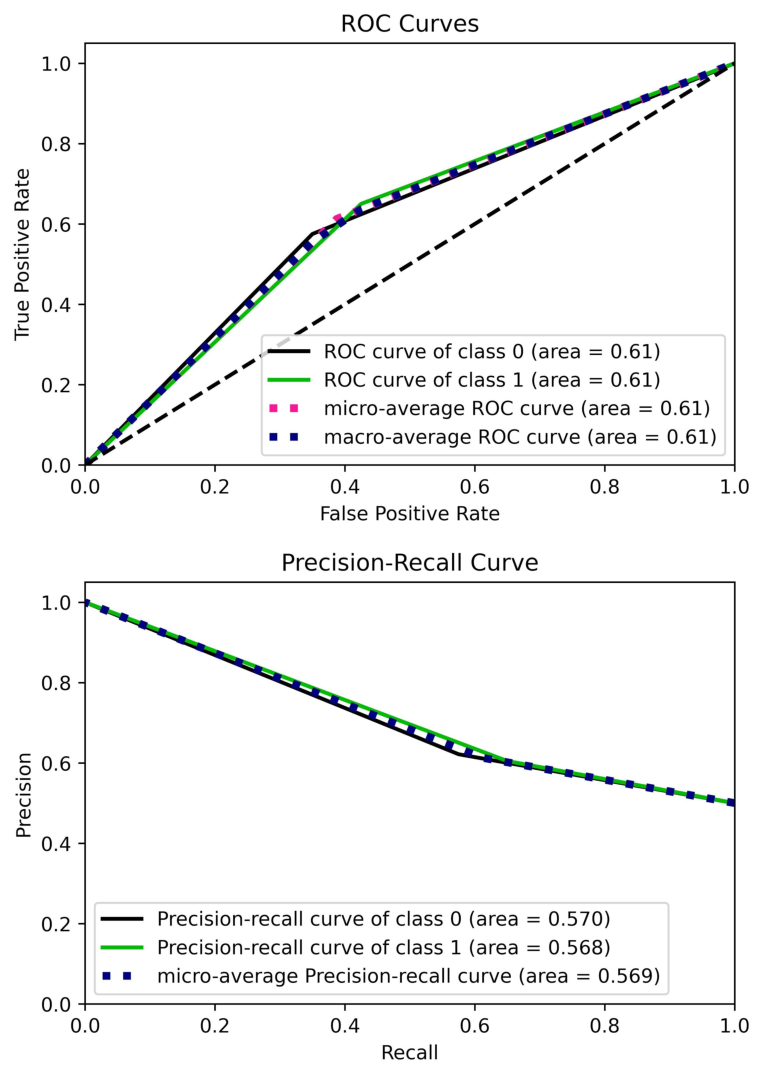
\includegraphics[width=0.4\textwidth, keepaspectratio]{points_roc.pdf}\label{fig:add_roc}}
\subfloat[Confusion Matrix]{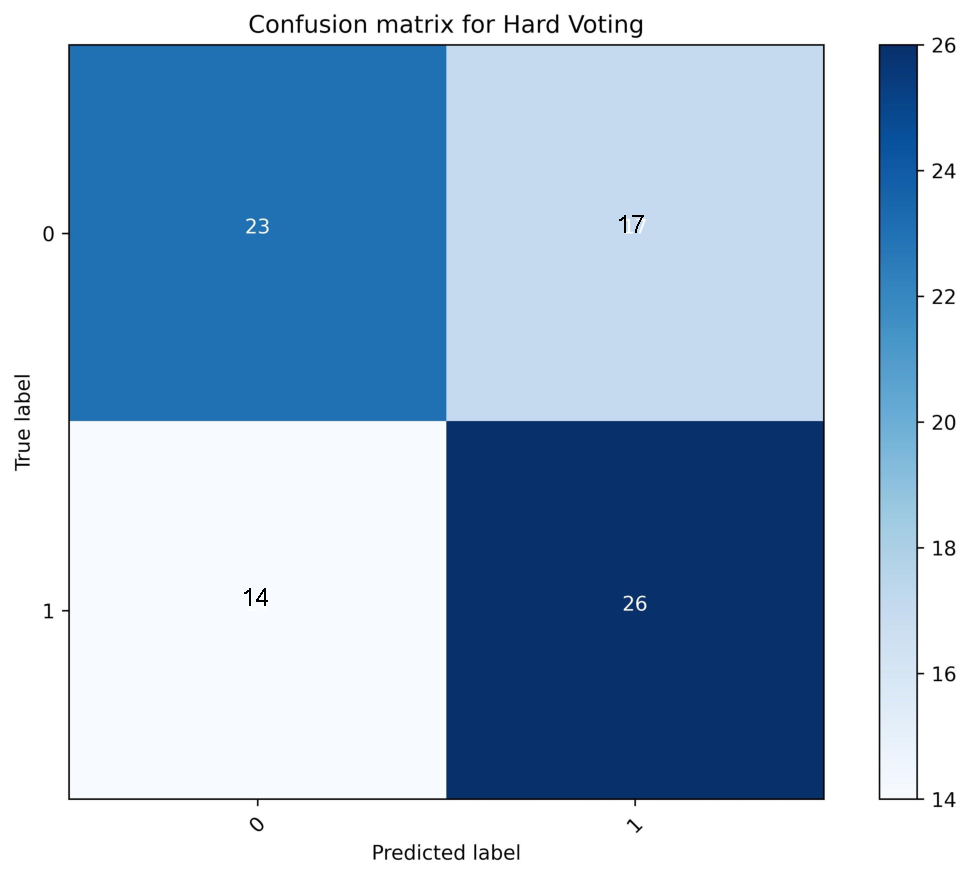
\includegraphics[width=0.4\textwidth,keepaspectratio]{points_cm.pdf}\label{fig:add_cm}}
\caption[]{Results of Classification using 3D Points}
\label{fig:points}
\end{figure}

While several experiments using PointNet are run on 3D points \cite{aoki2019pointnetlk, ge2018hand, garcia2016pointnet}, this was not applicable to the KM3NeT data. It could be because the points alone did not contain sufficient information for the network to learn from. As the network also randomly samples a fixed number of points per point cloud, it was likely that the relevant event hits were not selected by the random sampler. While it would have been computationally beneficial to successfully train a model without 3D meshes, these results provide justification for the mesh generation step in the pipeline. It was evident that the 3D meshes added the required level of detail necessary for PointNet to learn. 

\section{Alternate Pipeline: 4D PointNet}
\label{sec:additional-4d}
Experiments were also conducted to see if PointNet could learn from the \texttt{x, y, z, time} attributes at once, instead of generating three datasets. As 4D meshes are not technically feasible, the points were only pre-processed using radius-based outlier detection. The initial layers of the architecture were modified to accept 4 inputs (Appendix \ref{appendix-layers}). Training showed that the model was able to perform only slightly better than before. It achieved an accuracy of \textbf{57\%} with \textbf{78\%} recall for the positive class. Figure \ref{fig:4droc} shows low areas under the ROC and PR curves. The confusion matrix in Figure \ref{fig:4dcm} indicates that the classifier was better at classifying event timeslices over noise. 

\begin{figure}[ht!]   
\centering
\subfloat[ROC and PR curves]{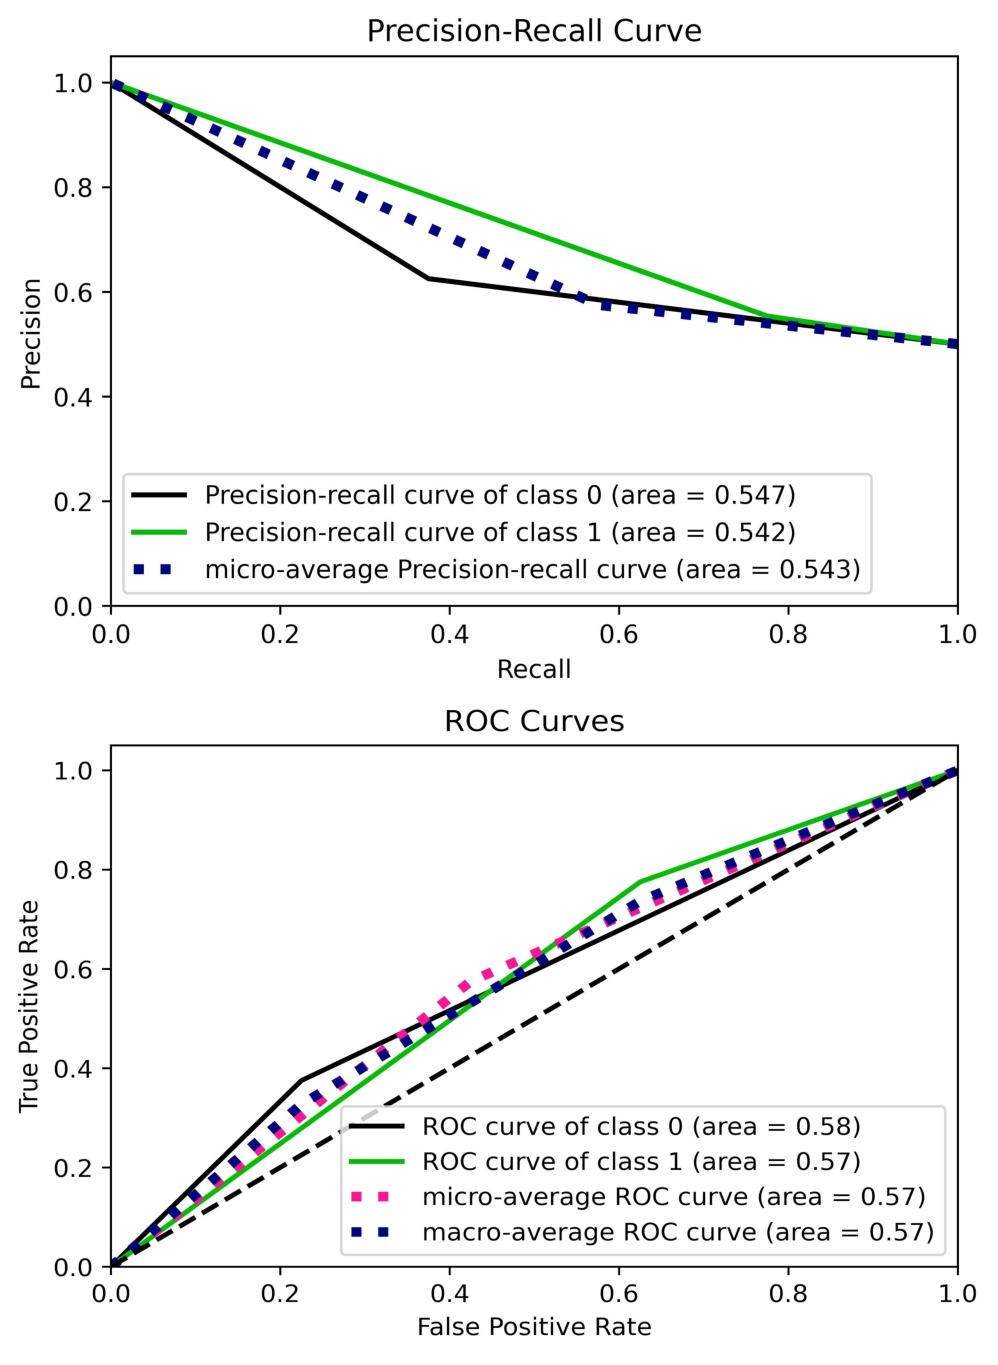
\includegraphics[width=0.4\textwidth, keepaspectratio]{4d_roc.pdf}\label{fig:4droc}}
\subfloat[Confusion Matrix]{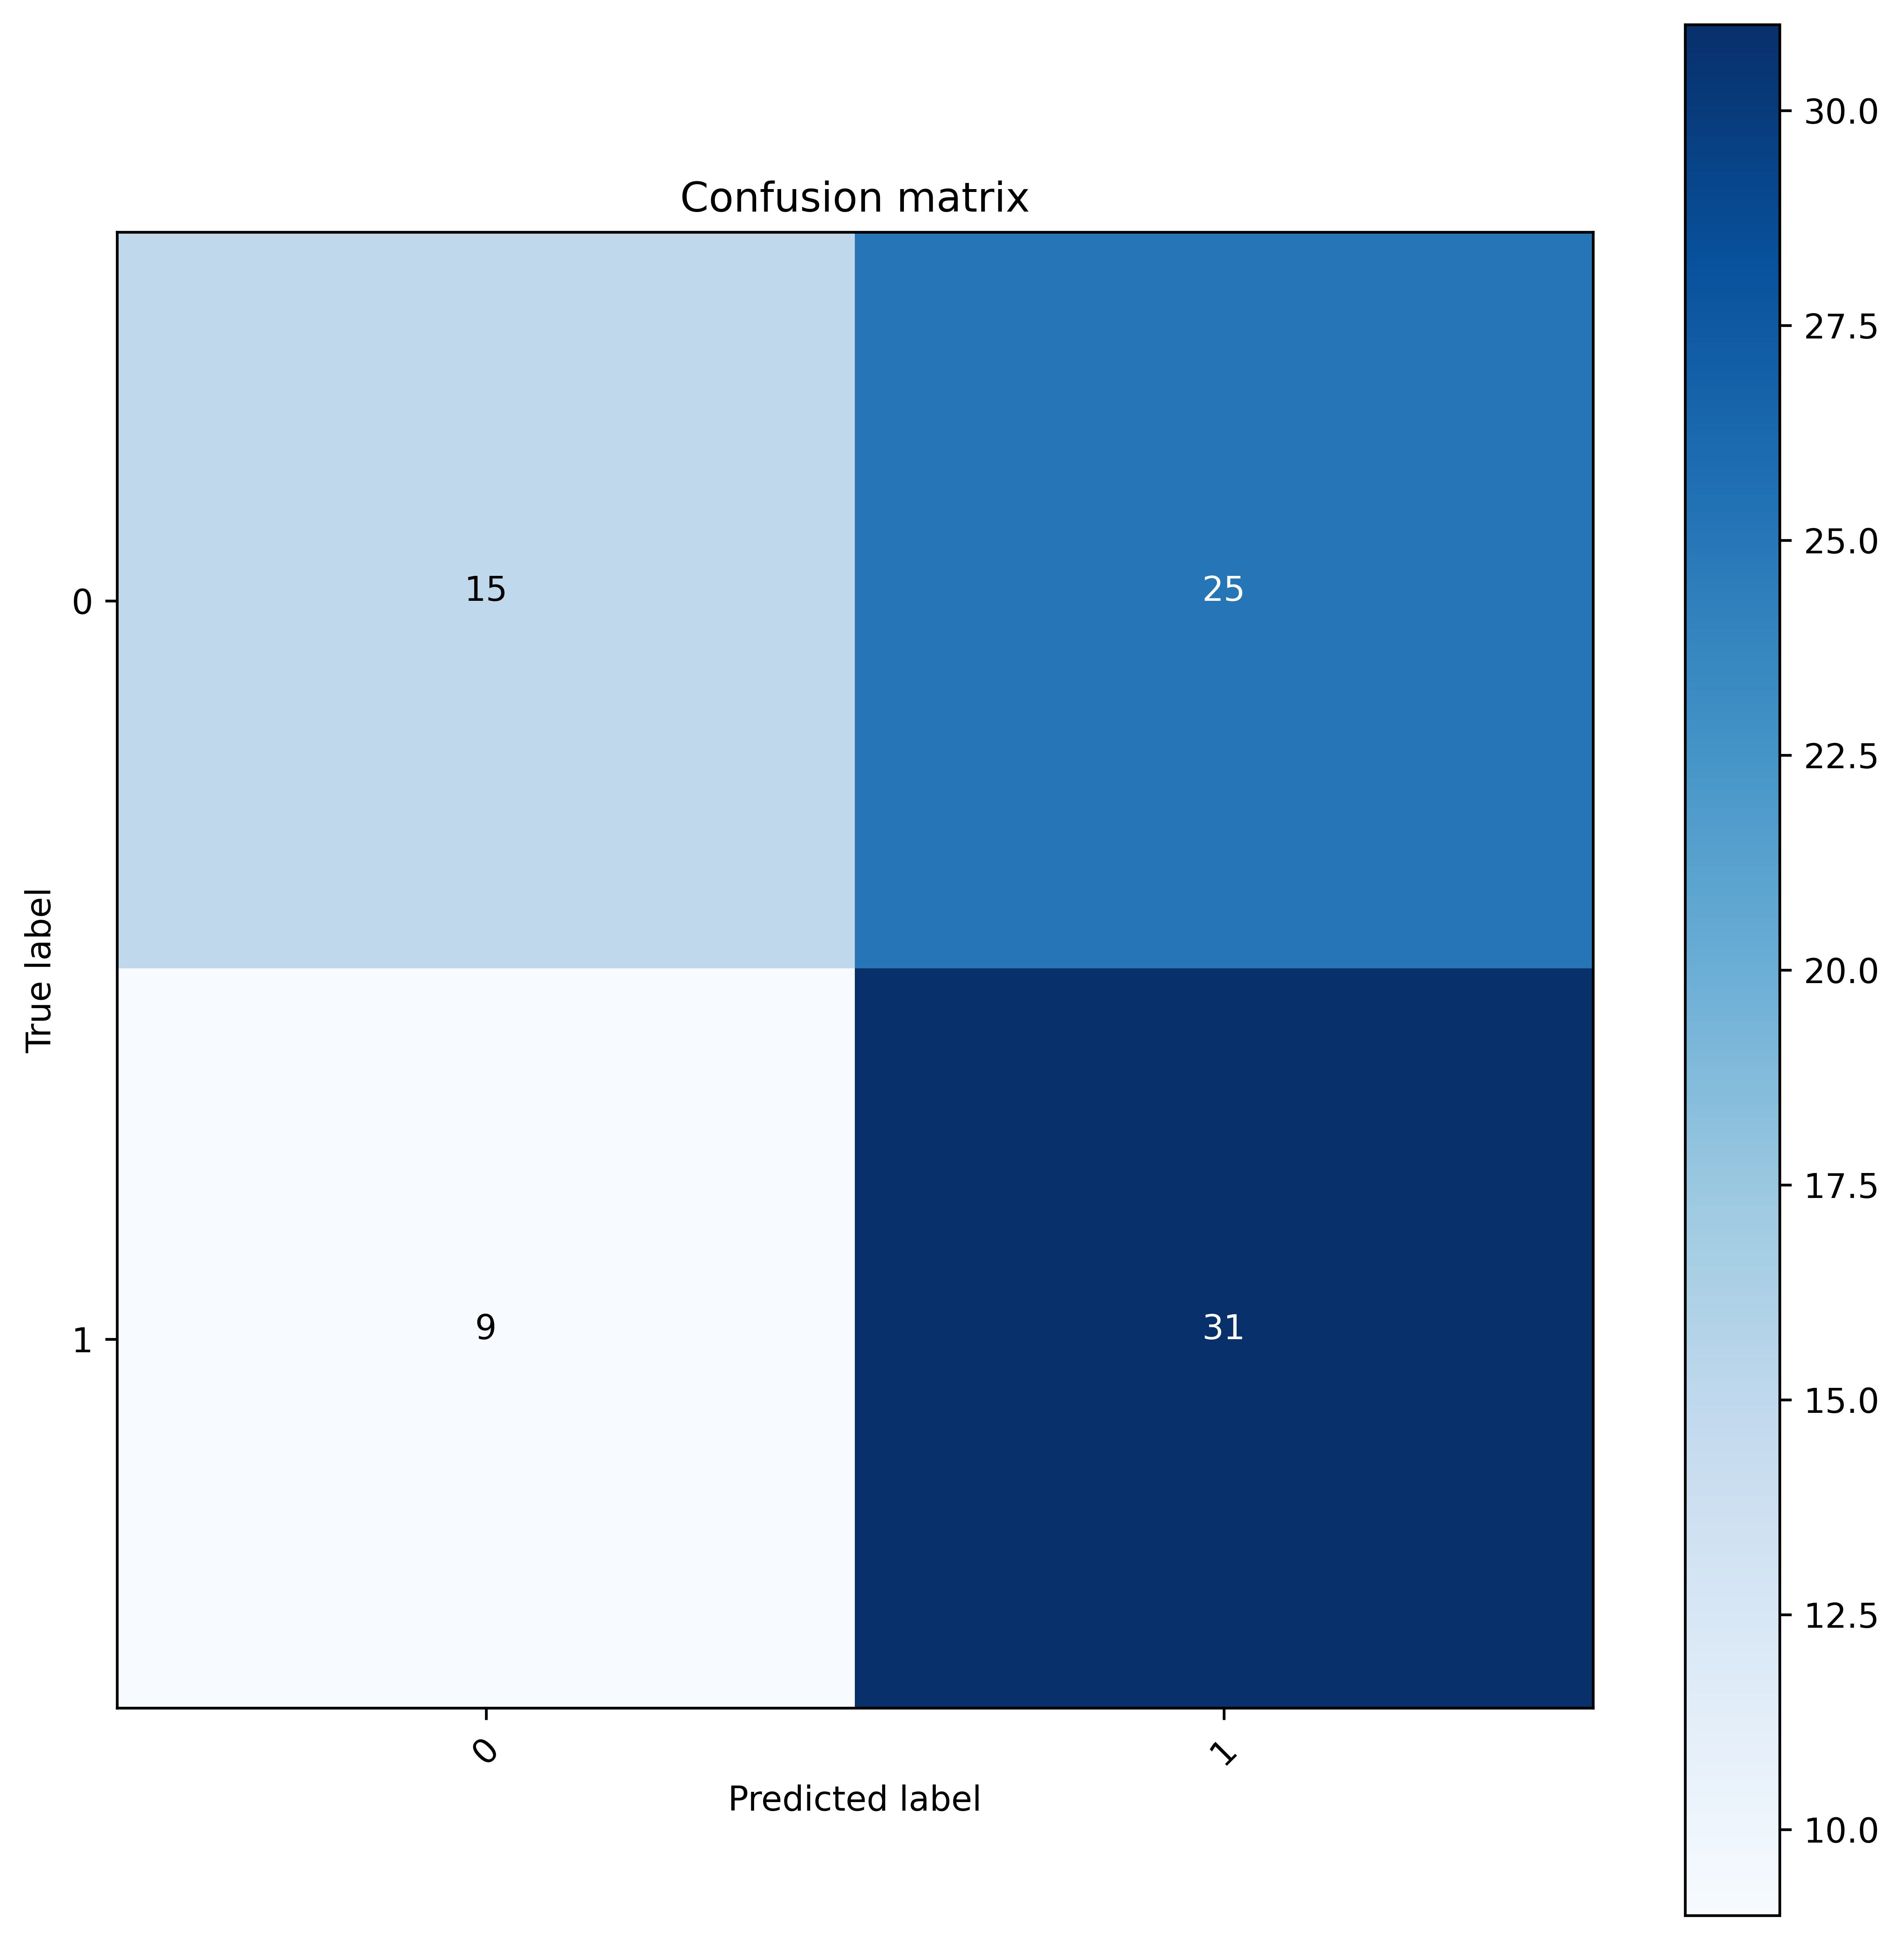
\includegraphics[width=0.4\textwidth,keepaspectratio]{4d_cm}\label{fig:4dcm}}
\caption[]{Results of Classification using 4D Points}
\label{fig:4d}
\end{figure}

\section{Regression Analysis for Energy Inference}
The final segment of the research question was focused on inferring energy values from timeslices classified as \texttt{class\_1} (\ref{sec:intro-research-questions}). Obtaining secondary properties such as the energy of an event is important as they can help identify lesser understood events such as decay of ark matter particles \cite{km3net_2017}. While PointNet can be theoretically used for regression tasks, there is no known research that demonstrate this yet \cite{qi2017pointnet}. PointNet was specifically built for object classification and segmentation tasks, so tuning the architecture for regression tasks would involve significant architectural changes. This indicated that a different architecture more suited for regression should be used instead of modifying PointNet. Additionally, the thesis pipeline started with the 3D coordinates and time values. However, these attributes were no longer represented by the same values when the point clouds were converted to 3D meshes. Thus, after classification, it would be challenging to map the 3D meshes to their respective energy values and proceed with training for regression. Due to these reasons, building a model for regression was more appropriate for a separate research project and was not attempted further. Instead, the remainder of the thesis investigated the inference of energy values using two non-linear techniques - decision trees and random forests bootstrapping. That is, experiments were not considered an extension of the classification pipeline and are only intended to lay the ground for future work.

\subsection{Data Preparation}

\begin{figure}[ht!]
    \centering
    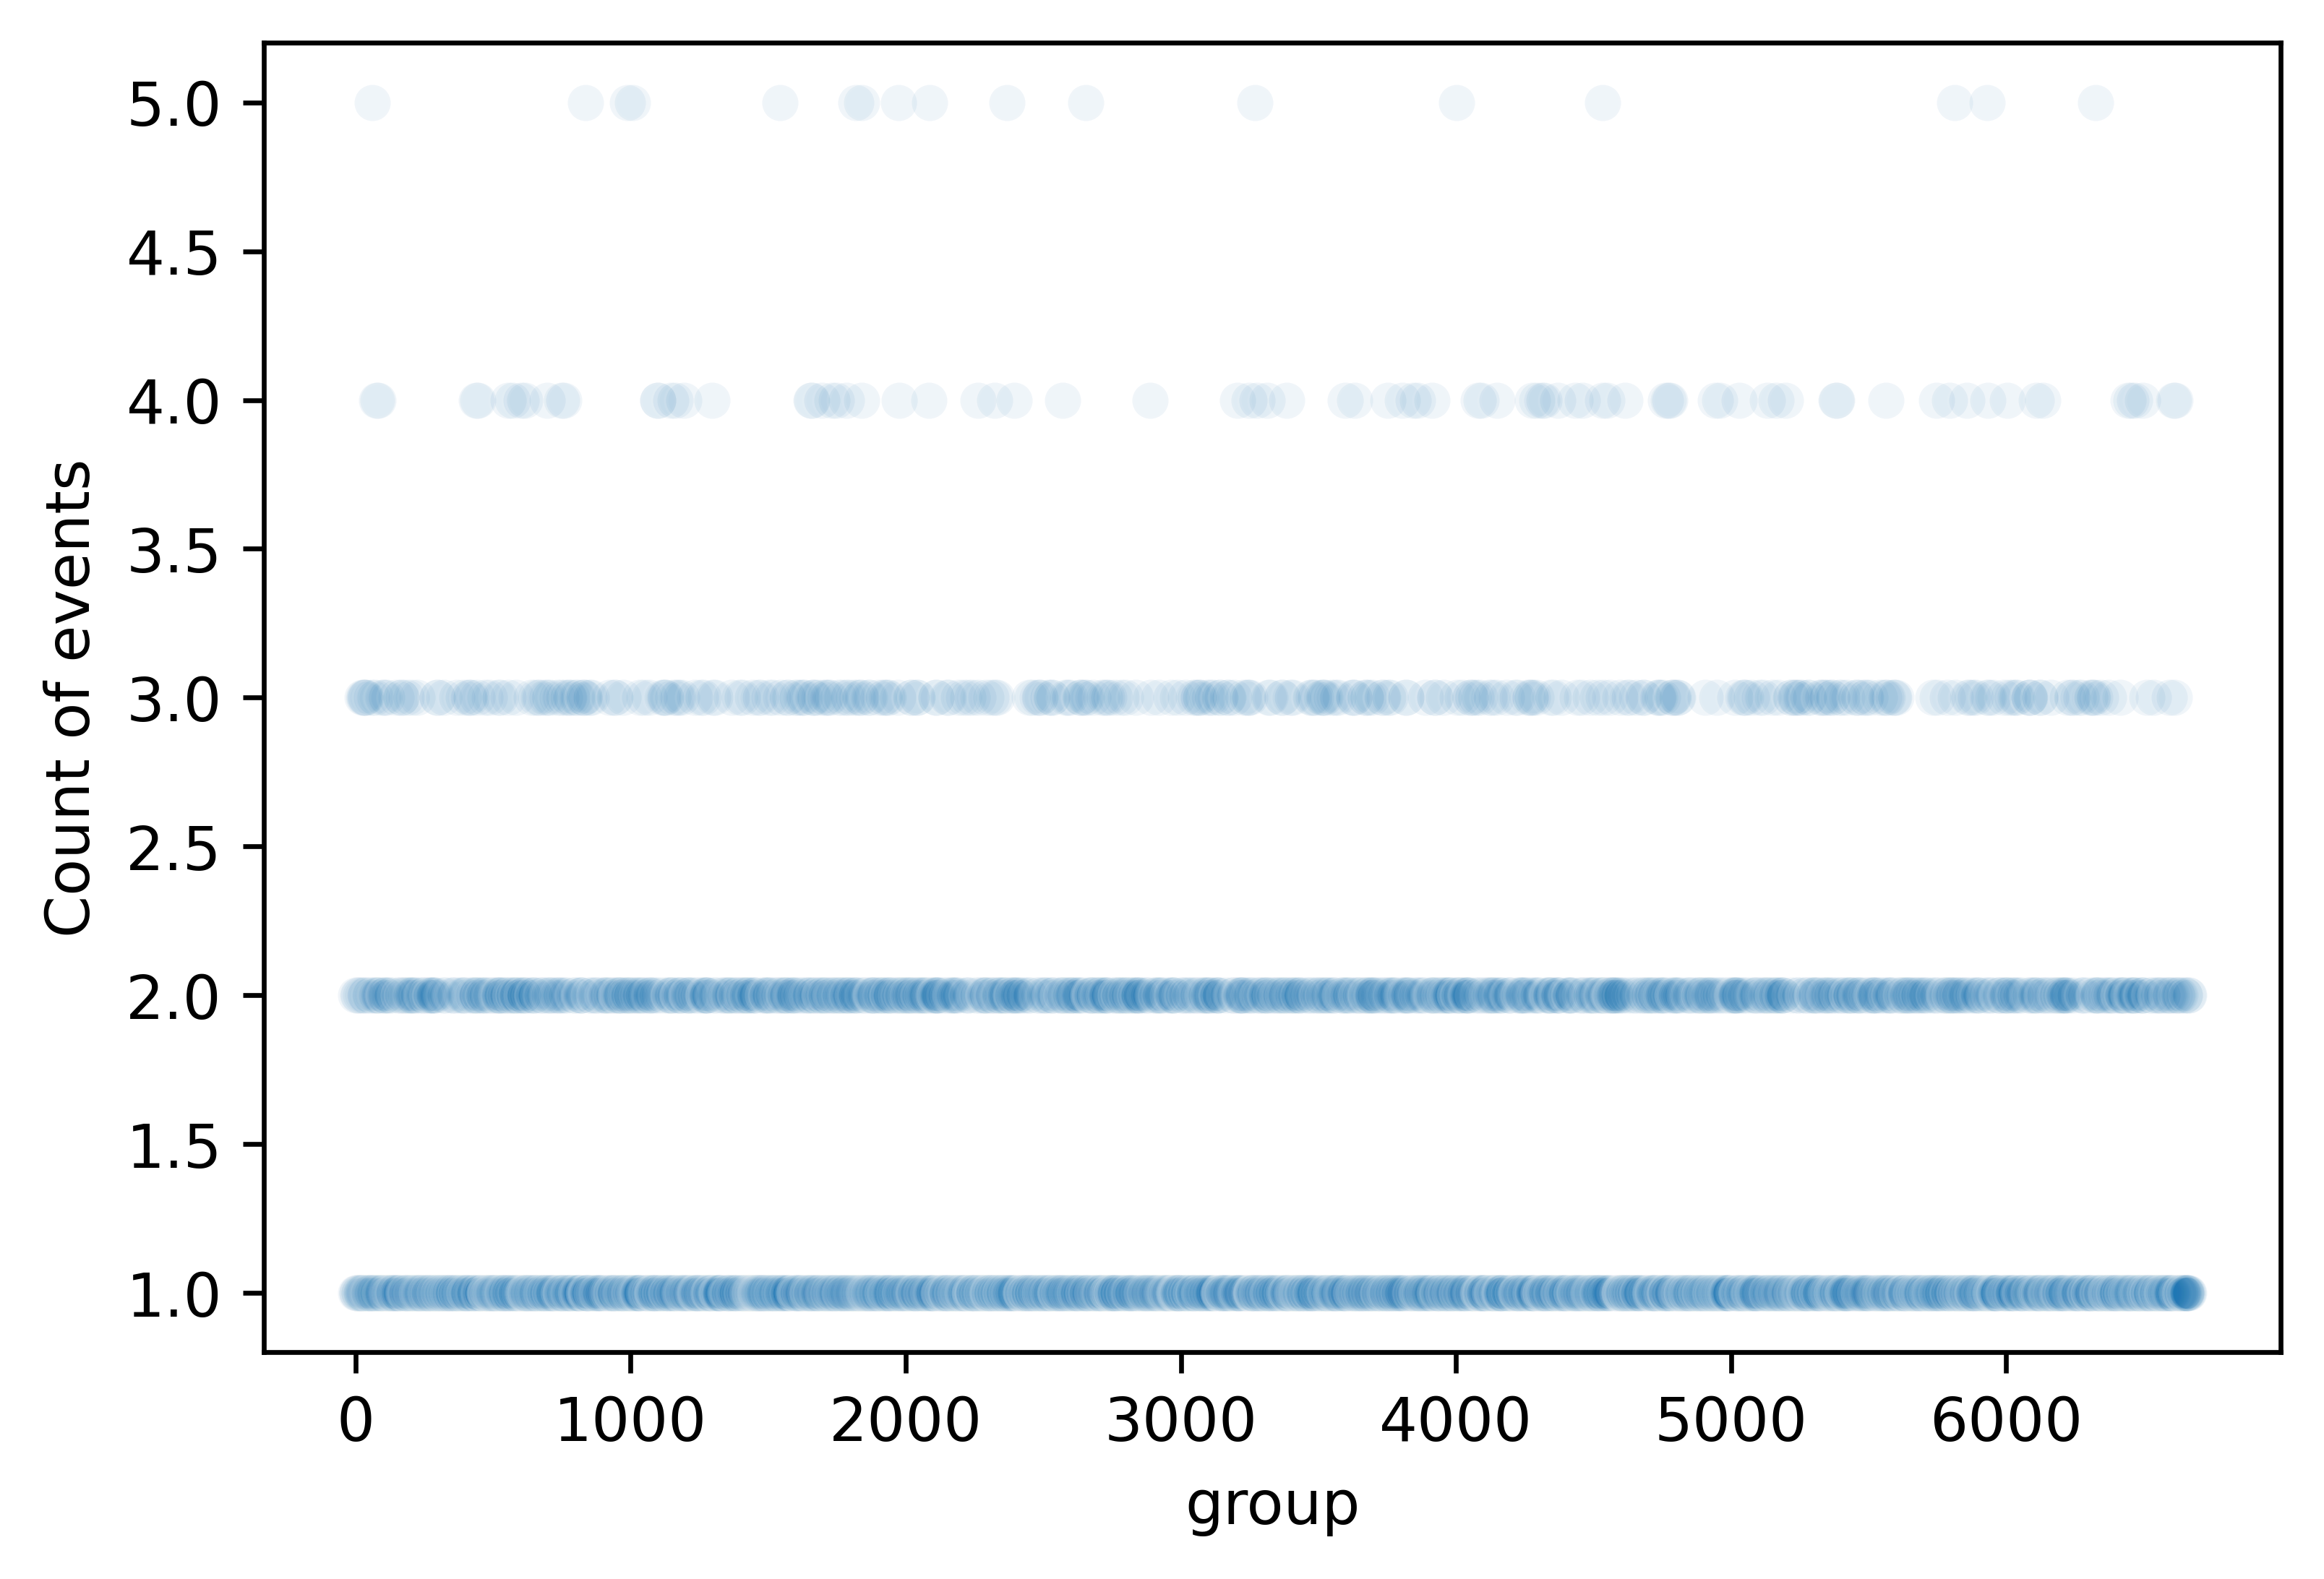
\includegraphics[width=0.7\textwidth, height=7cm, keepaspectratio]{energy_groups}
    \caption{Number of Energy Events Per Timeslice}
    \label{fig:energy_groups}
\end{figure}


HDF5 files containing \texttt{mc\_hits} and \texttt{mc\_info} tables were used (Section \ref{sec:exploration}). The energy events in the data were specifically in the range of 10 to 100 Gigaelectron-volts (GeV). \texttt{mc\_info} contained additional energy information corresponding to the event hits in the \texttt{mc\_hits} table. It contained energy values (\texttt{nu\_E}), the type of neutrino (\texttt{type}) and the start (\texttt{nu.hits.start}) and end times of the event hits (\texttt{nu.hits.end}). The \texttt{mc\_hits} and \texttt{mc\_info} tables were combined and grouped into timeslices of 15000 ns to obtain the complete events dataset with corresponding energy values. The scatter plot in Figure \ref{fig:energy_groups} shows the count of events that occurred within each timeslice. Most of the timeslices contained a single event while very few timeslices contained more than 3 events. 


Target and predictor variables were defined. \texttt{energy} was set to be the target variable that the model would predict. \texttt{pos\_x, pos\_y, pos\_z} and \texttt{time} were selected as the predictor variables that would be used to predict \texttt{energy}. The predictor variables were selected using uni-variate feature selection based on the \textit{k-best} scores from \textit{mutual information}. Mutual information (MI) measures the dependency between variables and is zero when the two random variables are independent \cite{kraskov2011erratum}. The correlation heatmap in Figure \ref{fig:correlation} and  Table \ref{tab:pearson}  show that \texttt{energy} had no significant relation with any other variables. 

\begin{figure}[ht!]
    \centering
    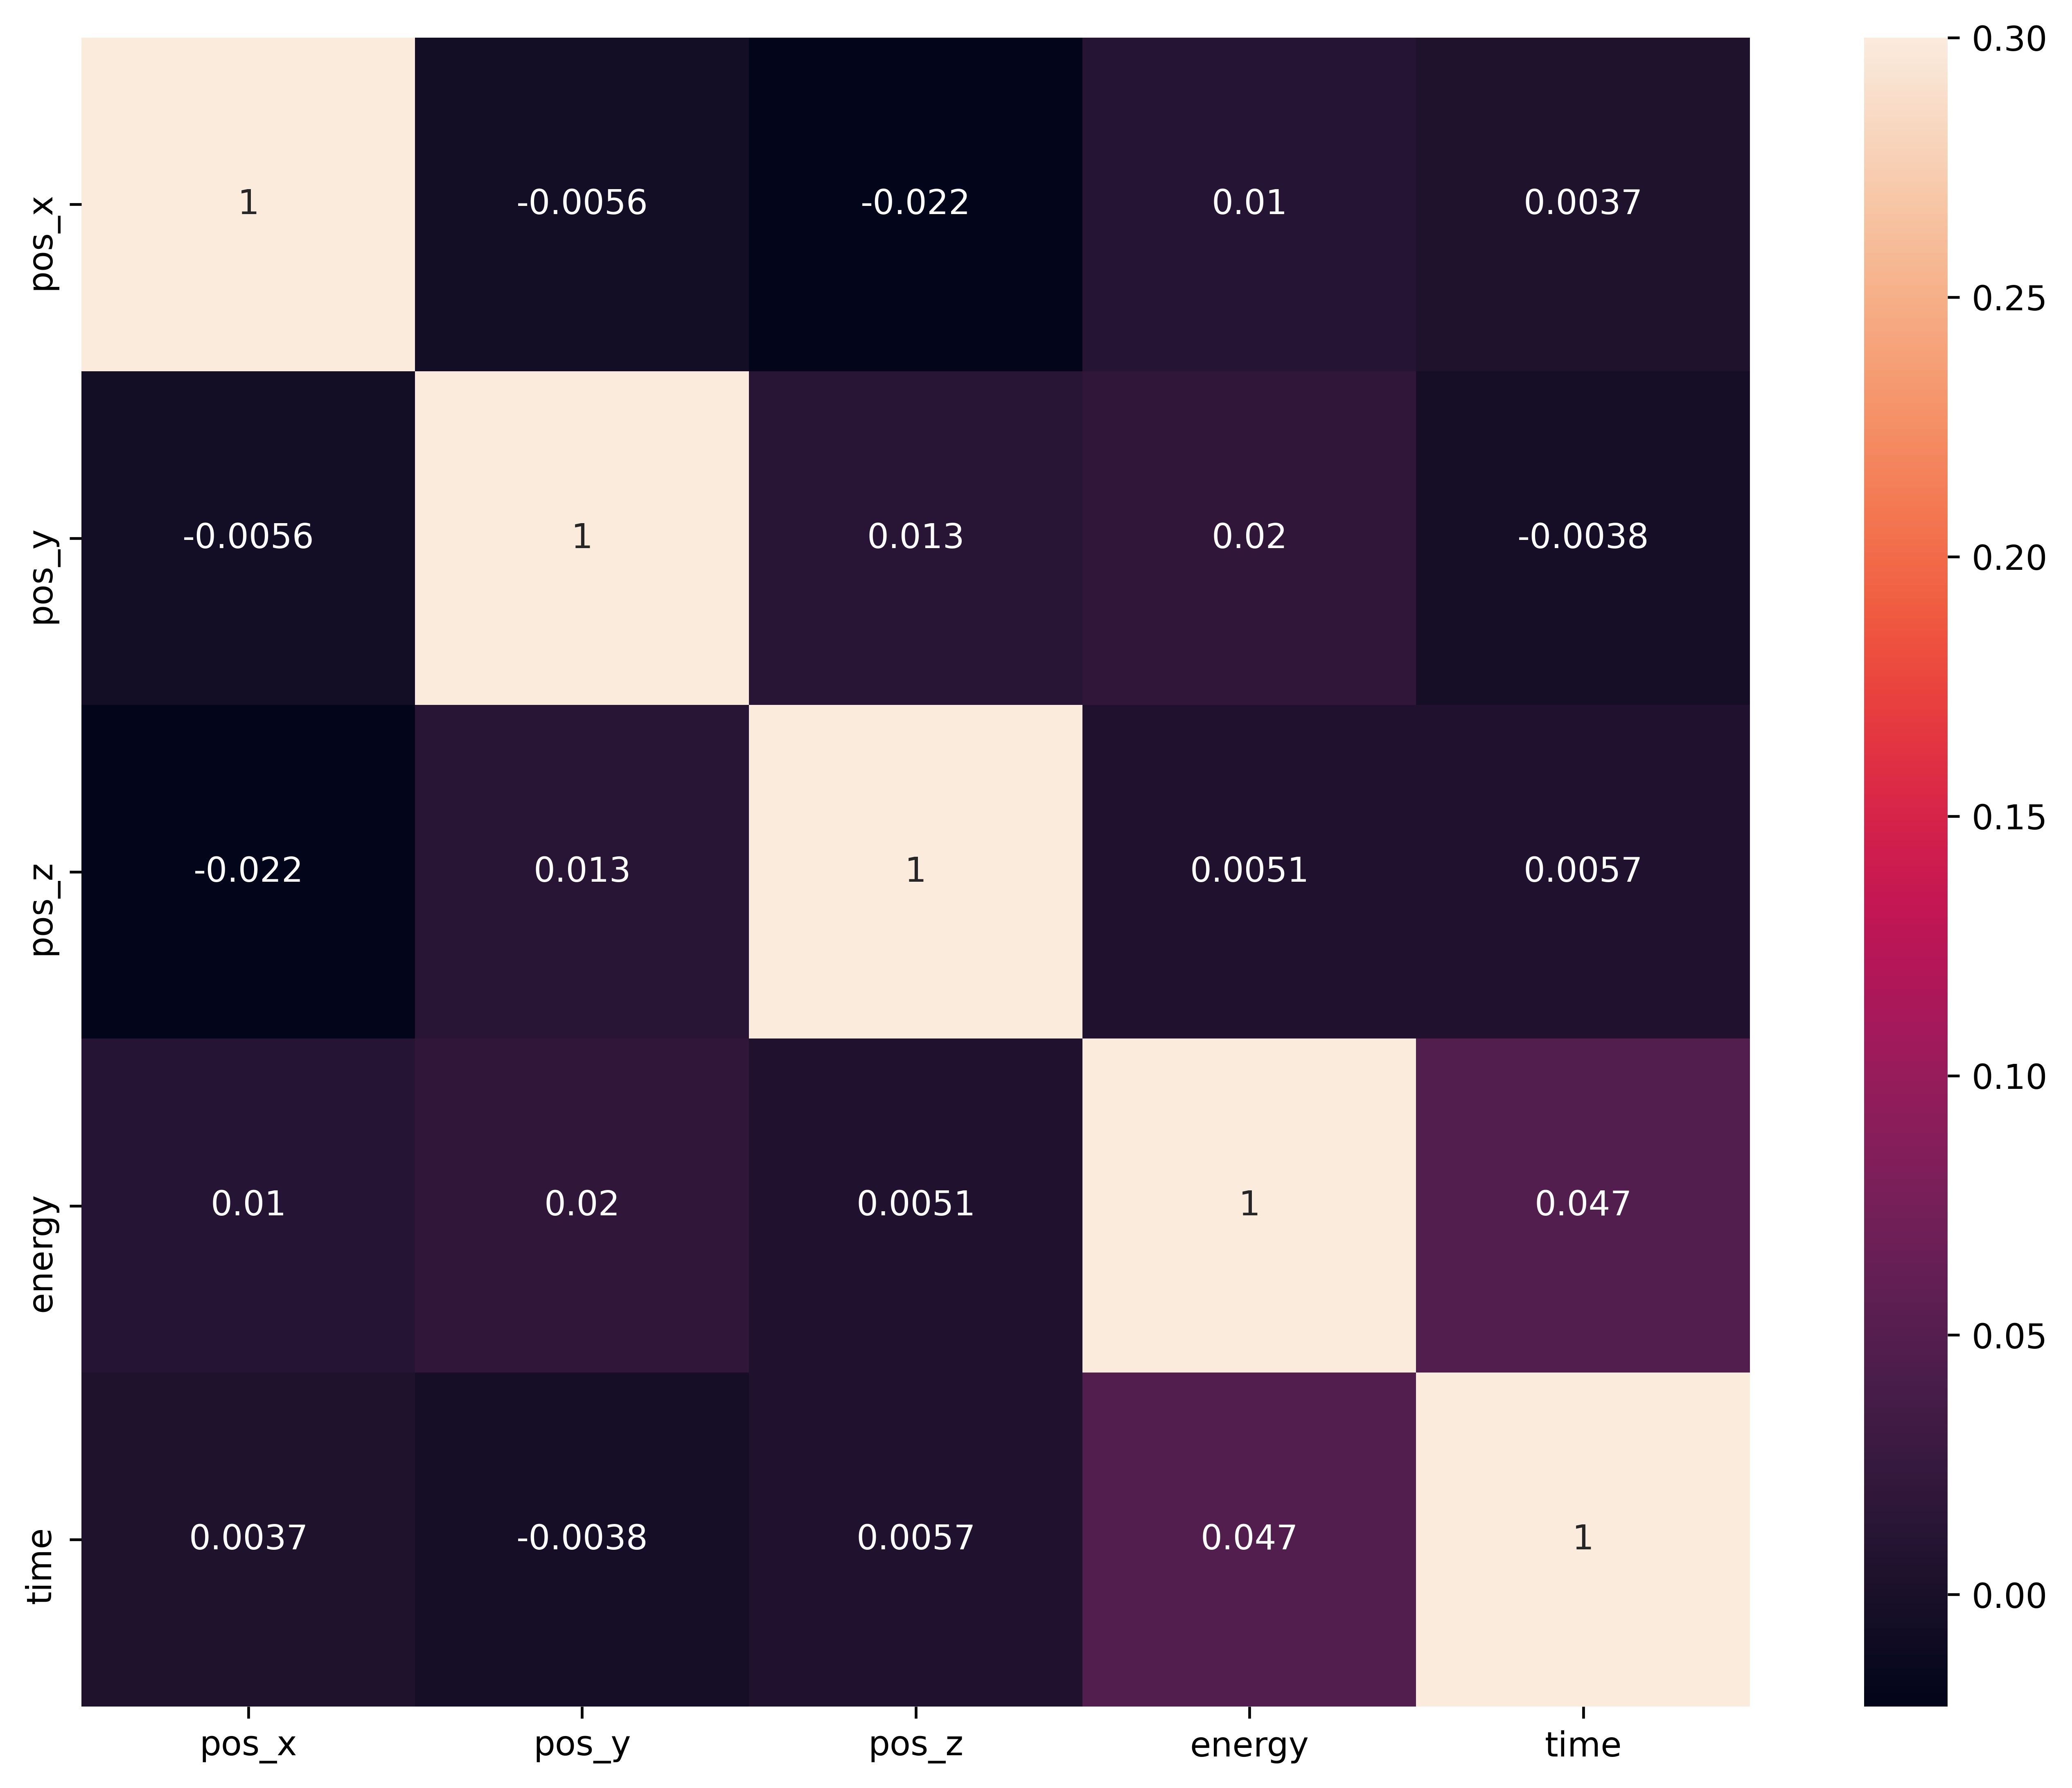
\includegraphics[width=0.7\textwidth, height=7cm, keepaspectratio]{correlation}
    \caption{Correlation Heatmap of the Events Dataset}
    \label{fig:correlation}
\end{figure}


\begin{table}[ht!]
    \centering
    \begin{tabular}{l c}
    \hline
        \texttt{energy} vs \texttt{time} & 0.05  \\
        \texttt{energy} vs \texttt{pos\_x}  & 0.01\\
        \texttt{energy} vs \texttt{pos\_y} & 0.02\\
        \texttt{energy} vs \texttt{pos\_z} & 0.005\\
    \hline
    \end{tabular}
    \caption{Correlation Coefficients: \texttt{energy} with \texttt{pos\_x, pos\_y, pos\_z} and \texttt{time}}
    \label{tab:pearson}
\end{table}

While all other key variables were found to have skewness close to 0, the target variable was  \textbf{0.88}. This indicated a high positive skew, affirmed via the non-normal density and probability plots in Figure \ref{fig:sl_proba}.

\begin{figure}[ht!]
    \centering
    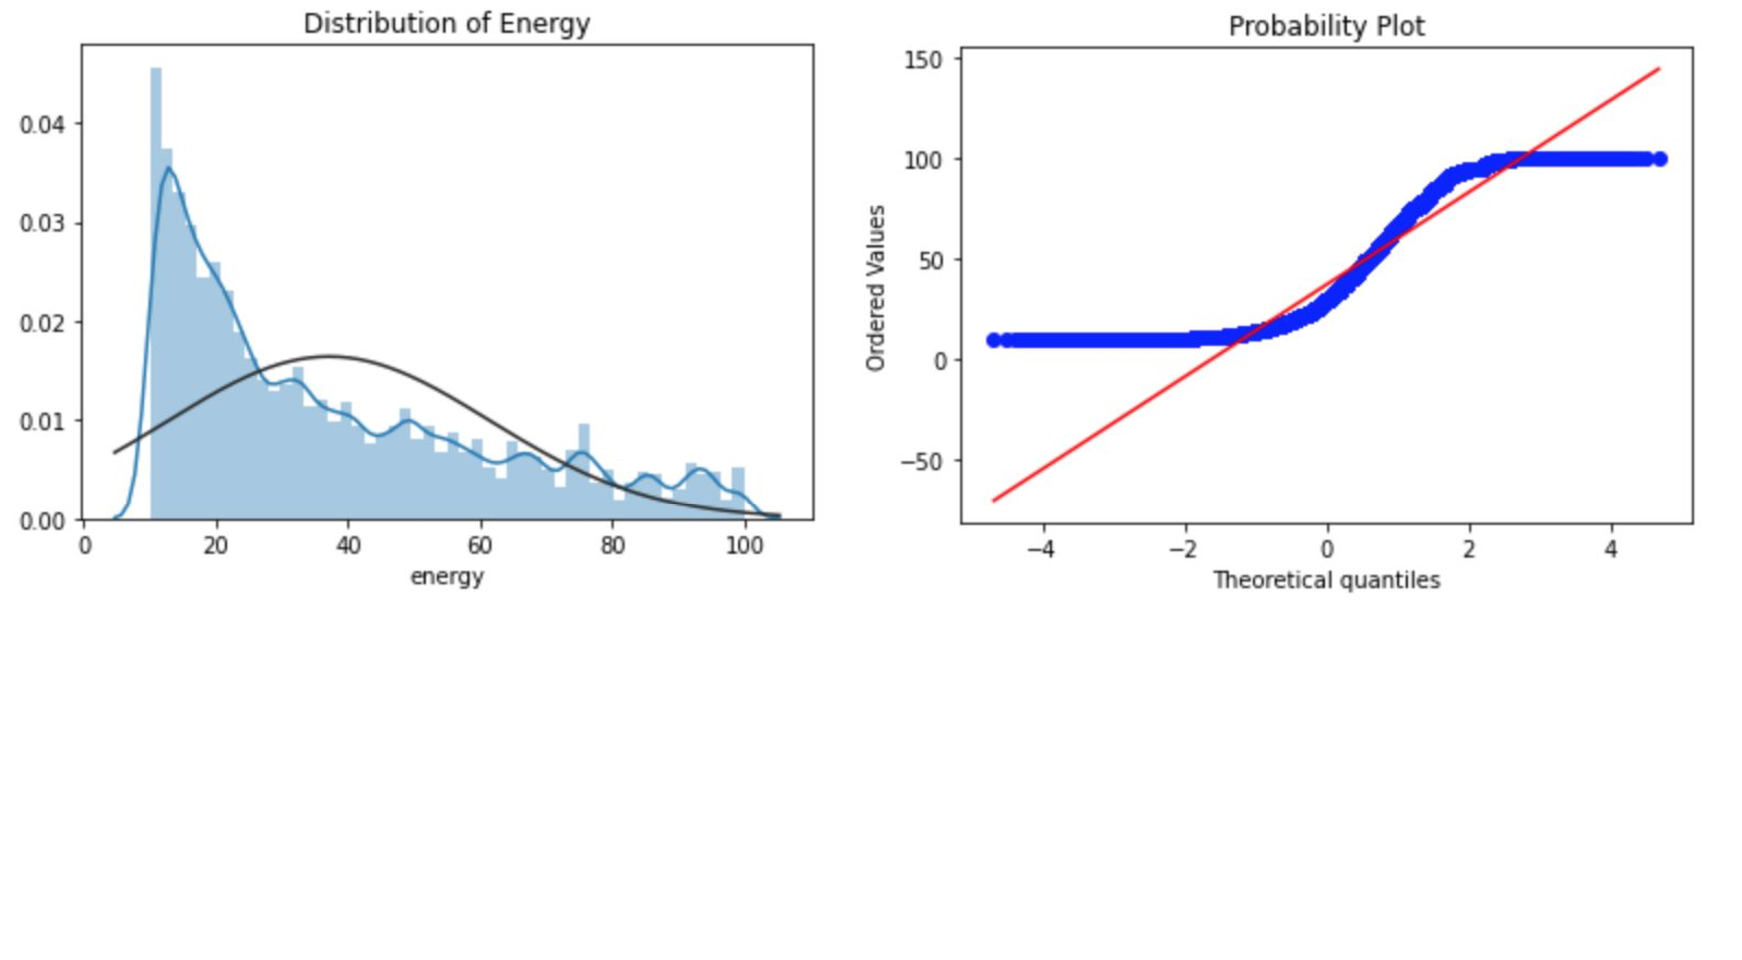
\includegraphics[width=\textwidth,keepaspectratio]{simple_linear_probability.pdf}
    \caption{Density and Probability Plot}
    \label{fig:sl_proba}
\end{figure}

It was evident that some transformation was required to bring the target as close to normal as possible. Three types of transformation functions were applied - \textit{log}, \textit{squared}, and \textit{Box-Cox}, and results were compared \cite{osborne2002notes, ruppert1985data}. Log and squared transformations involve taking the logarithm and square roots respectively. Box-Cox transformation makes use of $\lambda$ to approximate the best fitting values for the data \cite{box1964analysis}.

\begin{equation}
    \begin{aligned}
        y =  \begin{cases}(\frac{x^{\lambda - 1})}{\lambda} ,  \forall  \lambda > 0  \\
              log(x),                   \forall  \lambda = 0
              \end{cases}
    \end{aligned}
\end{equation}


\begin{figure}[ht!]   
\centering
\subfloat[Log Transformation]{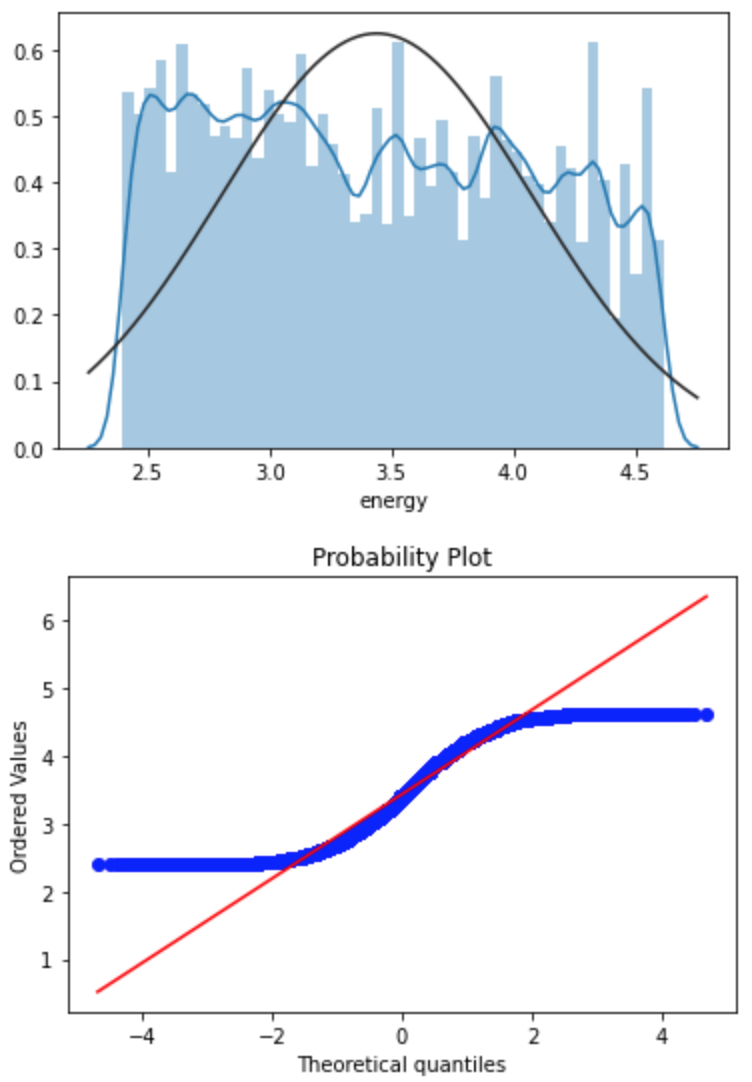
\includegraphics[width=0.3\textwidth, keepaspectratio]{log}\label{fig:log}}
\subfloat[Squared Transformation]{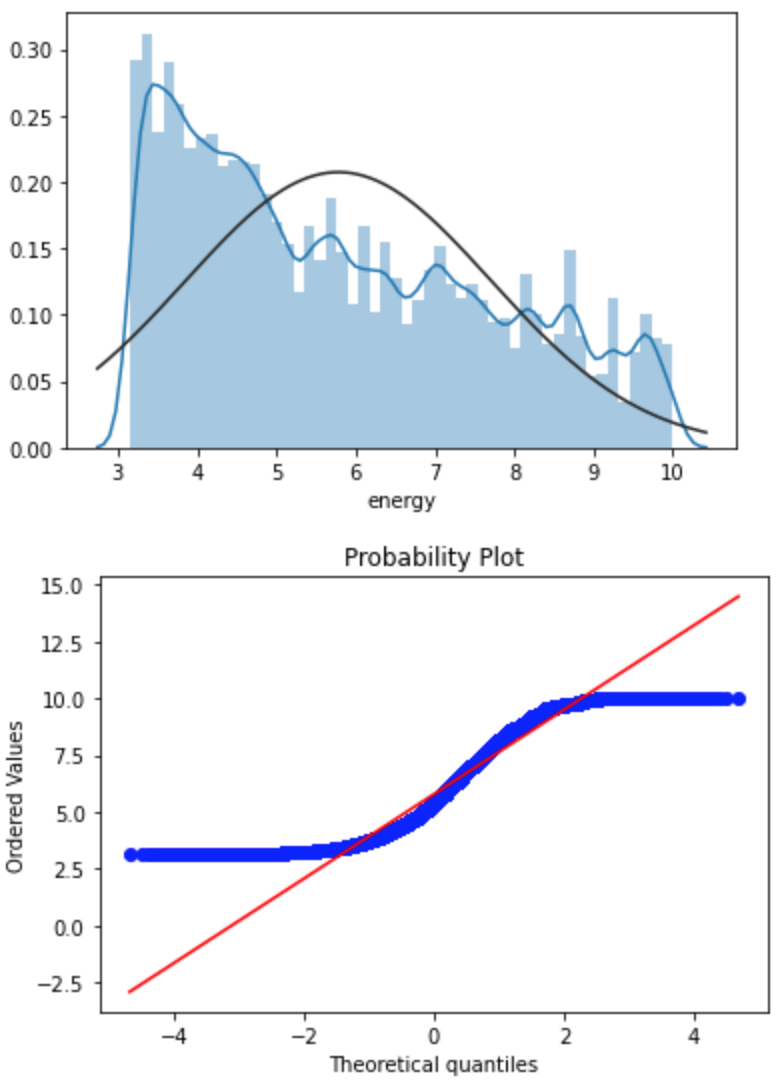
\includegraphics[width=0.3\textwidth, height=6.5cm]{sq}\label{fig:sq}}
\subfloat[Box-Cox Transformation]{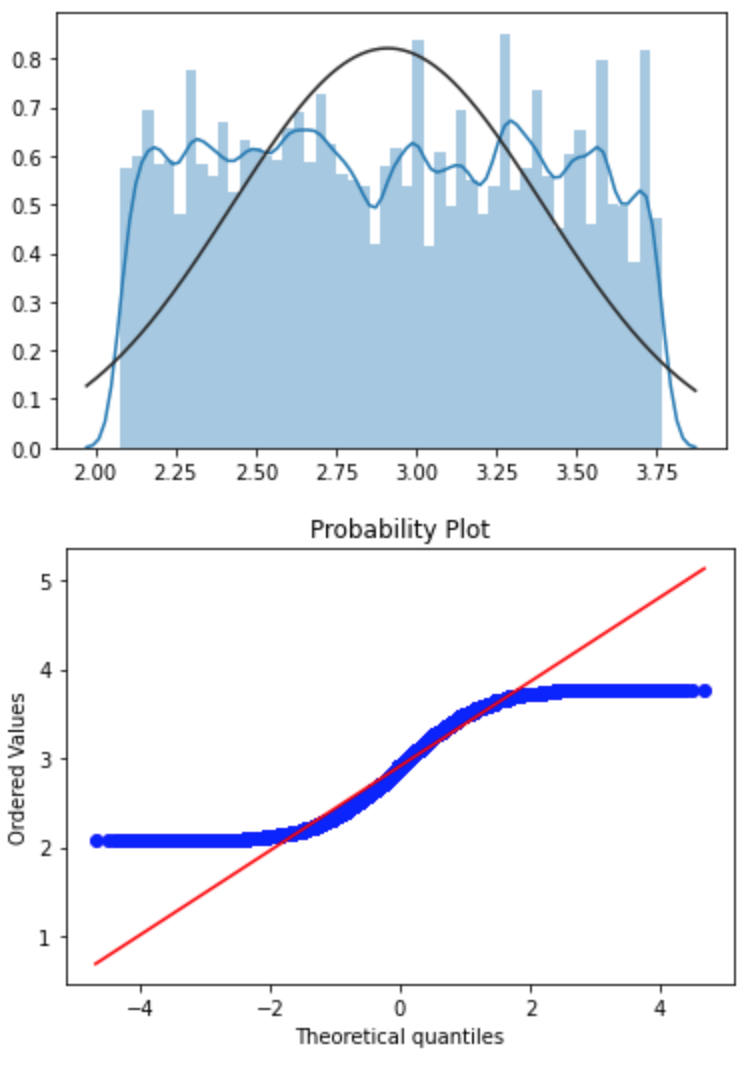
\includegraphics[width=0.3\textwidth, height=6.45cm]{boxcox}\label{fig:boxcox}}
\caption[]{Transformations of the Target Variable \texttt{energy}}
\label{fig:transformations}
\end{figure}

Figure \ref{fig:transformations} shows the application of each function. The skew after log transformation was \textbf{0.12} and the corresponding plot shows a more bell-shaped curve indicating some normalisation (Figure \ref{fig:log}). The squared transformation did not result in useful improvements, indicated by the still right skewed data (Figure \ref{fig:sq}), and a skew value of \textbf{0.49}. Better results were obtained from the Box-Cox transformation that had the lowest skew of \textbf{0.02} and the corresponding plot in Figure \ref{fig:boxcox} showed a distribution aligned towards normal. Thus the target variable was transformed using Box-Cox.

\begin{figure}[ht!]   
\centering
\subfloat[Training Data]{\includegraphics[width=0.33\textwidth, keepaspectratio]{energy_train}\label{fig:train}}
\subfloat[Testing Data]{\includegraphics[width=0.33\textwidth, keepaspectratio]{energy_test}\label{fig:test}}
\subfloat[Additional Evaluation Data]{\includegraphics[width=0.33\textwidth, keepaspectratio]{energy_hold}\label{fig:eval}}
\caption[]{Distribution of Energy for Events in Training, Testing and Additional Evaluation Data}
\label{fig:energy_train_test_eval}
\end{figure}


50 timeslices from the dataset were randomly selected and kept aside for evaluation. The dataset was then split into training and testing components using a 66/34 split. Figure \ref{fig:energy_train_test_eval} shows the distribution of energy corresponding to events within the training, testing and additional evaluation data. Here, energy values were binned into 10 groups for a simpler visualisation. Sub-figures \ref{fig:train} and \ref{fig:test} show that both the training set and testing set contained a good balance between low and high energy events. The additional evaluation set in Sub-figure \ref{fig:eval} shows that most of the events had low energy, especially under 30 GeV. This indicated that the model could be evaluated against a challenging dataset since lower energy events do not have many hits associated with them. 


Standard regression metrics, Mean Squared Error (MSE) and coefficient of determination (R2) were chosen for performance measurement. MSE indicates the average squared difference between the estimated value and actual value \cite{montgomery2012introduction}. R2 metric provides an indication of the goodness of fit of a set of predictions to the actual values \cite{montgomery2012introduction}. In order to get a complete unbiased picture, both metrics were used.

 
\subsection{Decision Trees Regressor}
Decision Trees are a non-parametric, supervised learning method where the model makes predictions by learning simple decision rules inferred from data features \cite{breiman1984classification}. They were chosen because they require very little data preparation and  are computationally efficient \cite{breiman1984classification}. 342,920 samples were selected for training and 146,966 samples were used for testing. Sklearn's \texttt{DecisionTreeRegressor} was used to initialise a decision tree, with parameters based on experimentation. Tree depth was \texttt{20} and the minimum samples required to be at a leaf node was set to be \texttt{1}. 

\begin{table}[ht!]
    \centering
    \begin{tabular}{l c c c}
    \hline
        & Training & Testing & Additional \\
    \hline
    MSE & 100.3 &  116.3 & 269.0 \\
    R2  & 0.83 & 0.80 & 0.31 \\ 
    \hline
    \end{tabular}
    \caption{Decision Tree Regression Metrics}
    \label{tab:decision_scores}
\end{table}

MSE and R2 were used as metrics of performance (Table \ref{tab:decision_scores}) for the training, testing and additional 50 timeslices. The model obtained a \textbf{0.80} R2 score on the testing data indicating a good fit. However, the MSE value on the testing set was \textbf{116}, which indicated large errors. After training and testing, the model was evaluated on the 50 timeslices. Here, it showed an even larger magnitude of error of \textbf{200} and R2 scores of \textbf{0.32}. Therefore, while the model performed well during training and testing, with no data leakage, it had lower performance on the 50 holdout timeslices. With no data leak in place, this has to be attributed to the complexity of the examples provided and overfitting.

\begin{figure}[ht!]   
\centering
\subfloat[Testing Data]{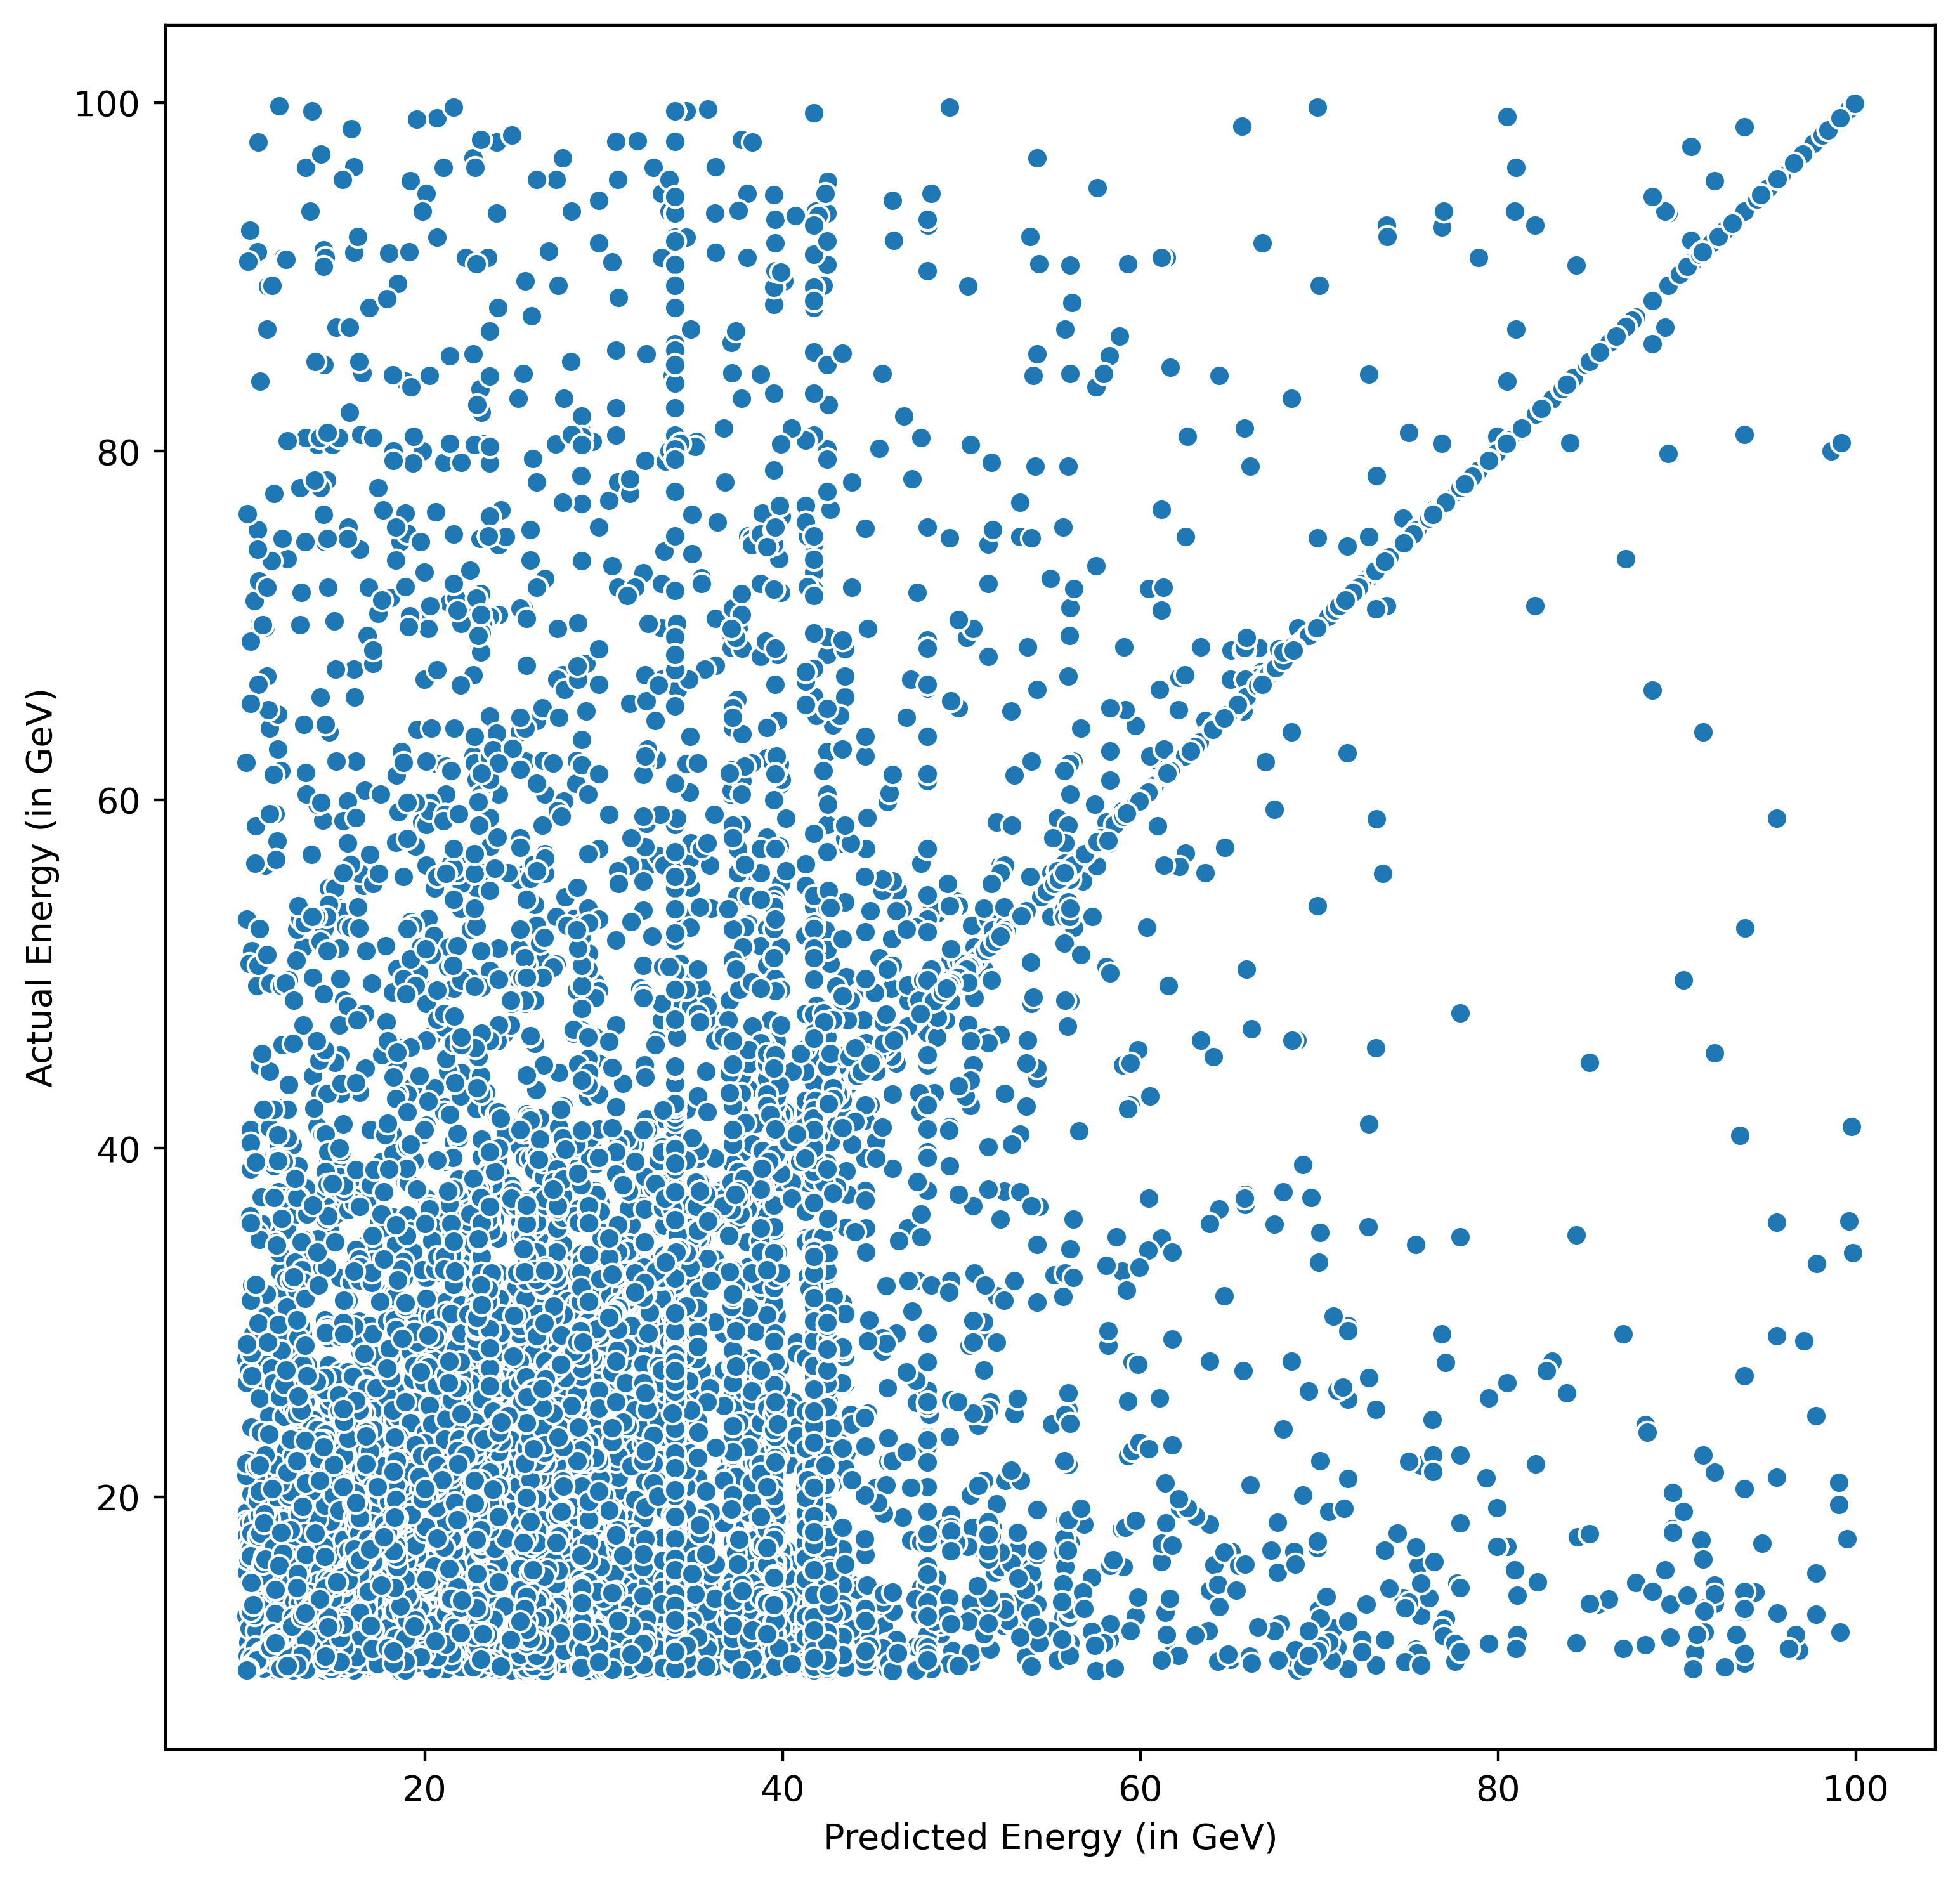
\includegraphics[width=0.44\textwidth,height=5cm, keepaspectratio]{results_dt}\label{fig:test_dt}}
\subfloat[50 Evaluation Timeslices]{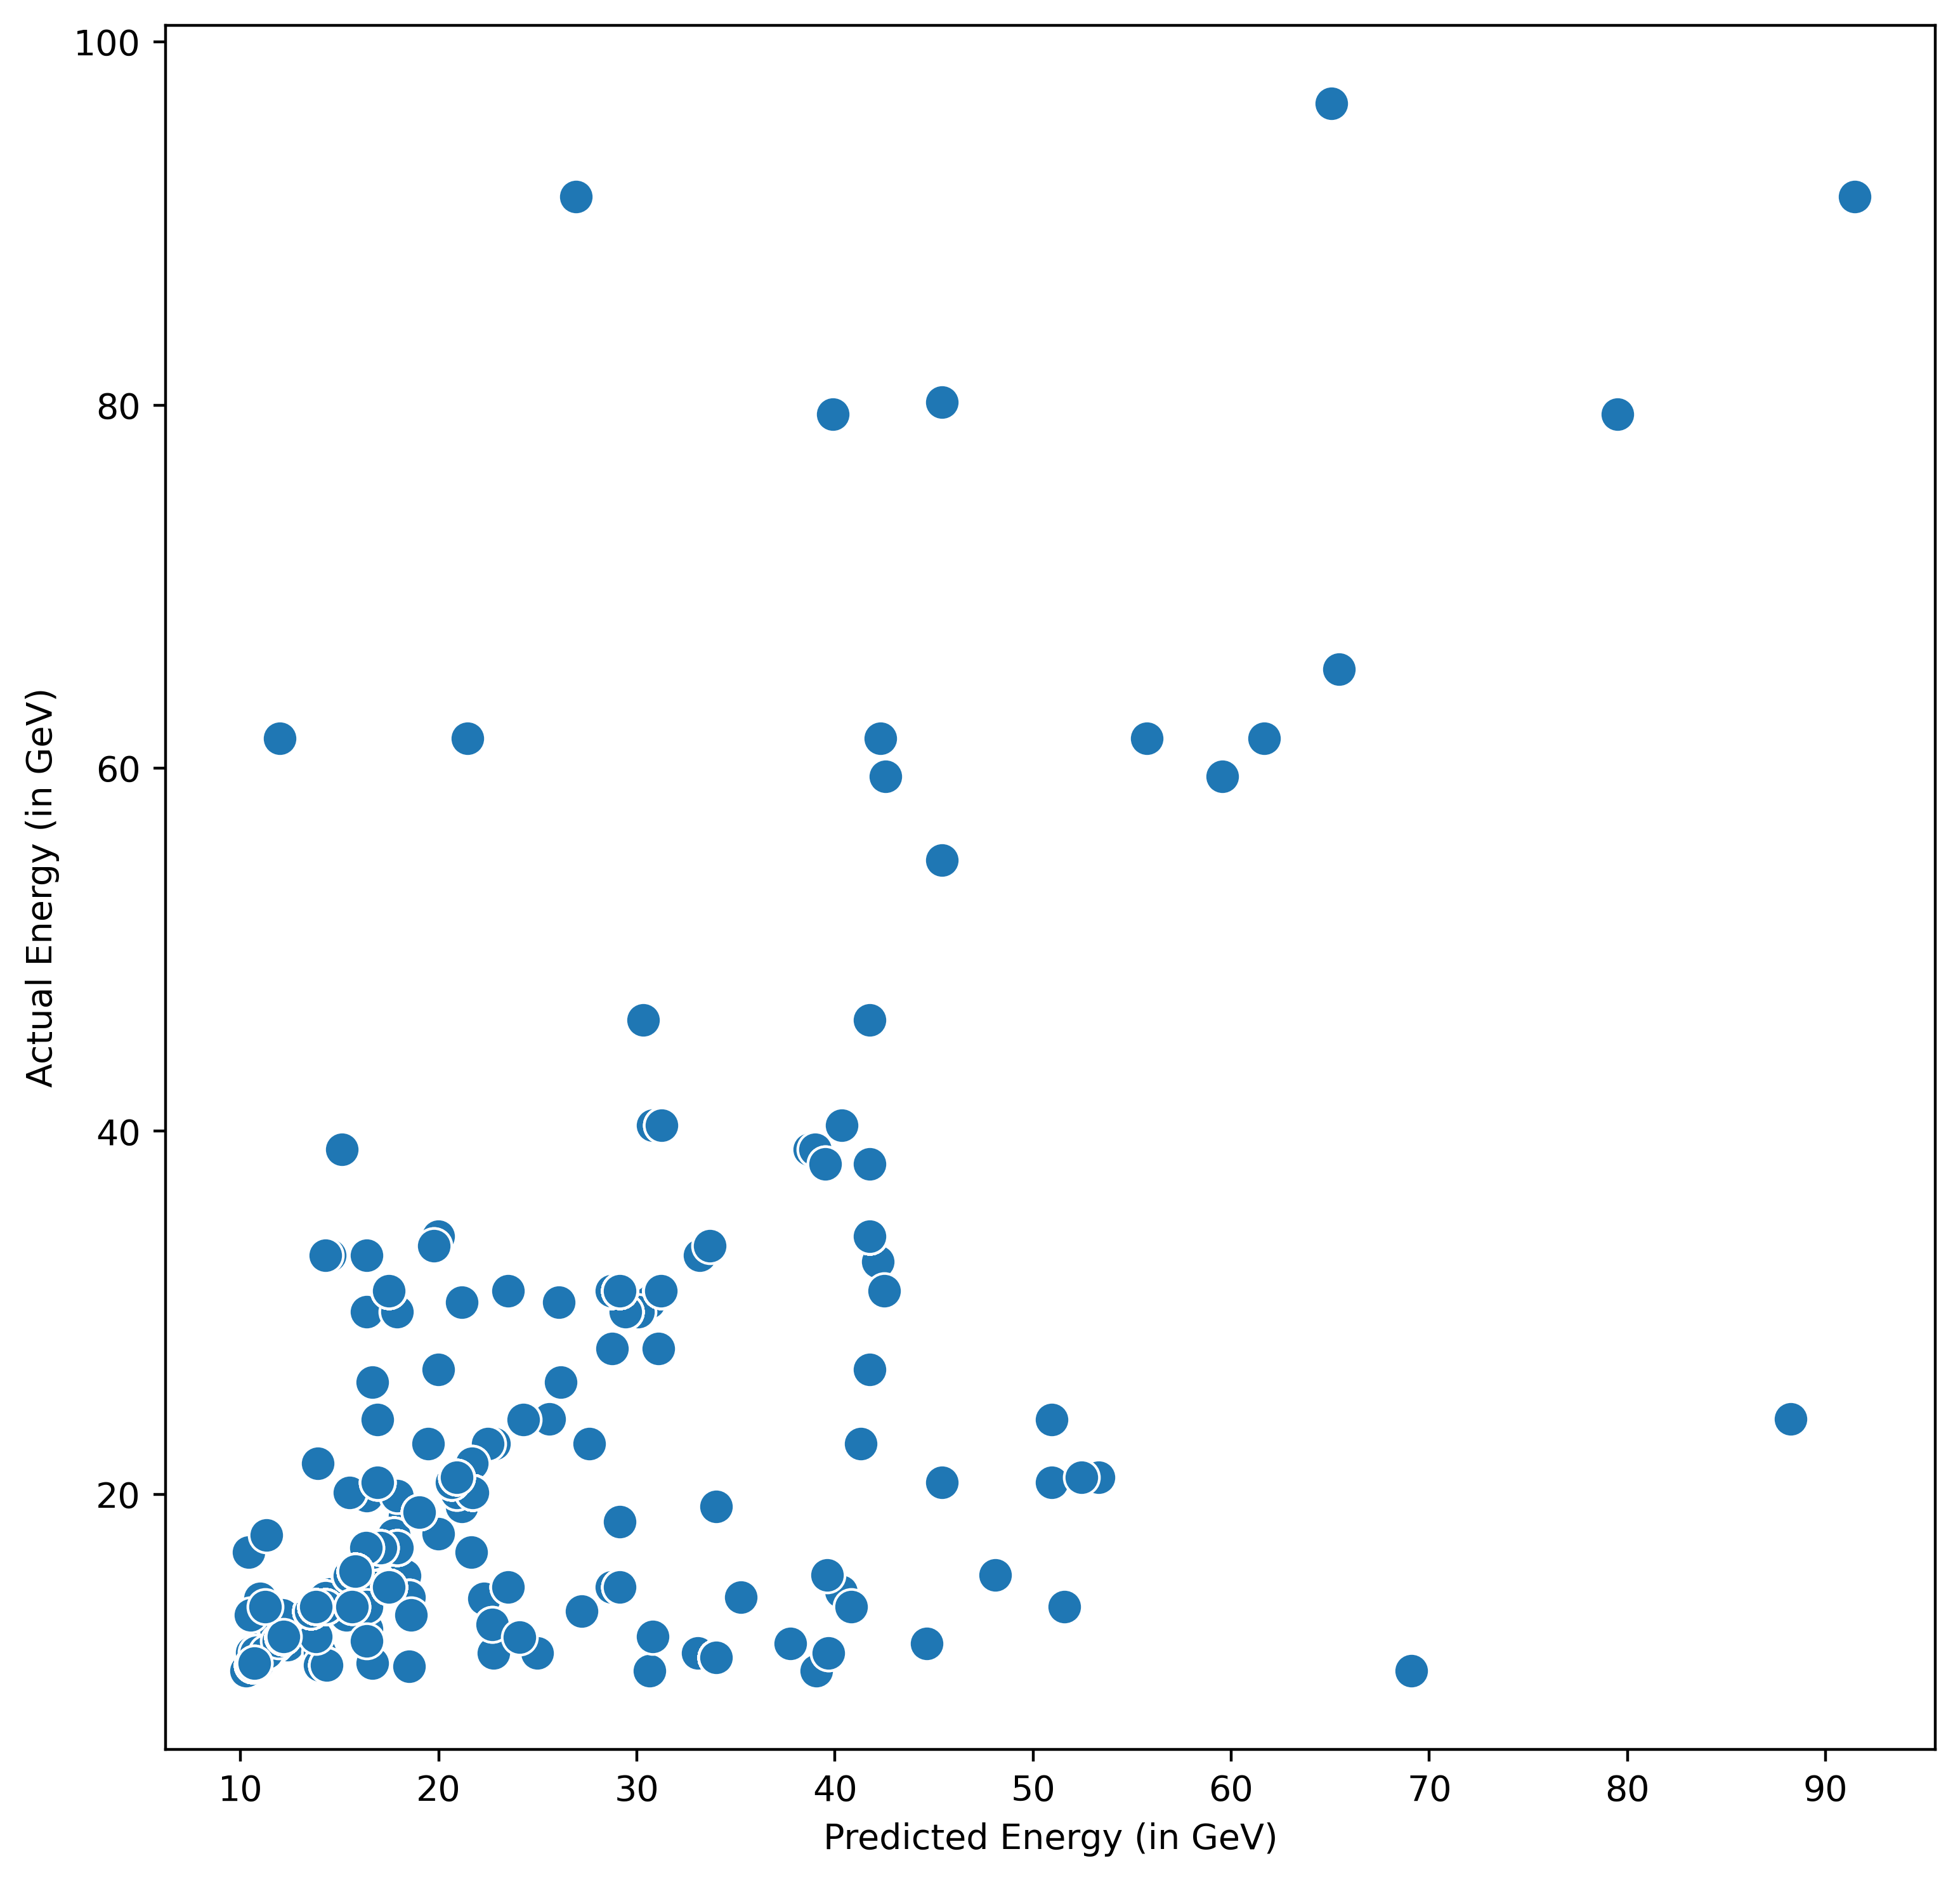
\includegraphics[width=0.44\textwidth,height=5cm, keepaspectratio]{results_eval_dt}\label{fig:eval_dt}}
\caption[]{Decision Trees Regressor: Actual vs Predicted Energy Values on Testing and Evaluation Data}
\label{fig:results_dt}
\end{figure}

Figure \ref{fig:results_dt} shows the plot of actual versus predicted energy values on the testing and evaluation data. The model was better at predicting lower energy values. High incidence of points in the upper left triangle of Sub-figure \ref{fig:test_dt} further indicate that the model was biased towards predicting lower energy values for higher energy events.

\subsection{Random Forest Bootstrapping Regressor}
A random forest is an estimator that fits a number of decision trees on various sub-samples of the dataset and uses averaging to improve the predictive accuracy and control over-fitting. With the same train/test setup, \texttt{50} trees were chosen to build the model. 

\begin{table}[ht!]
    \centering
    \begin{tabular}{l c c c}
    \hline
        & Training & Testing & Additional \\
    \hline
    MSE & 2.6 &  15.93 & 79.8 \\
    R2  & 0.99 & 0.97 & 0.80 \\ 
    \hline
    \end{tabular}
    \caption{Random Forest (Bootstrap Aggregation)  Metrics}
    \label{tab:rf_scores}
\end{table}

This time, both the MSE and R2 results were very promising (Table \ref{tab:rf_scores}). MSE showed lower errors of \textbf{15.93} on the testing data and the high R2 value of \textbf{0.97} showed good model fit. However, there is evidence of overfitting due to the difference between MSE scores during training and test. Additionally, evaluation on the 50 data samples gave significantly better results than the other models. While the MSE indicated higher errors, the R2 value of \textbf{0.80} showed a good fit with the data. The model was able to predict energy up to 12.138 GeV for events containing only 32 hits. 

\begin{figure}[ht!]   
\centering
\subfloat[Testing Data]{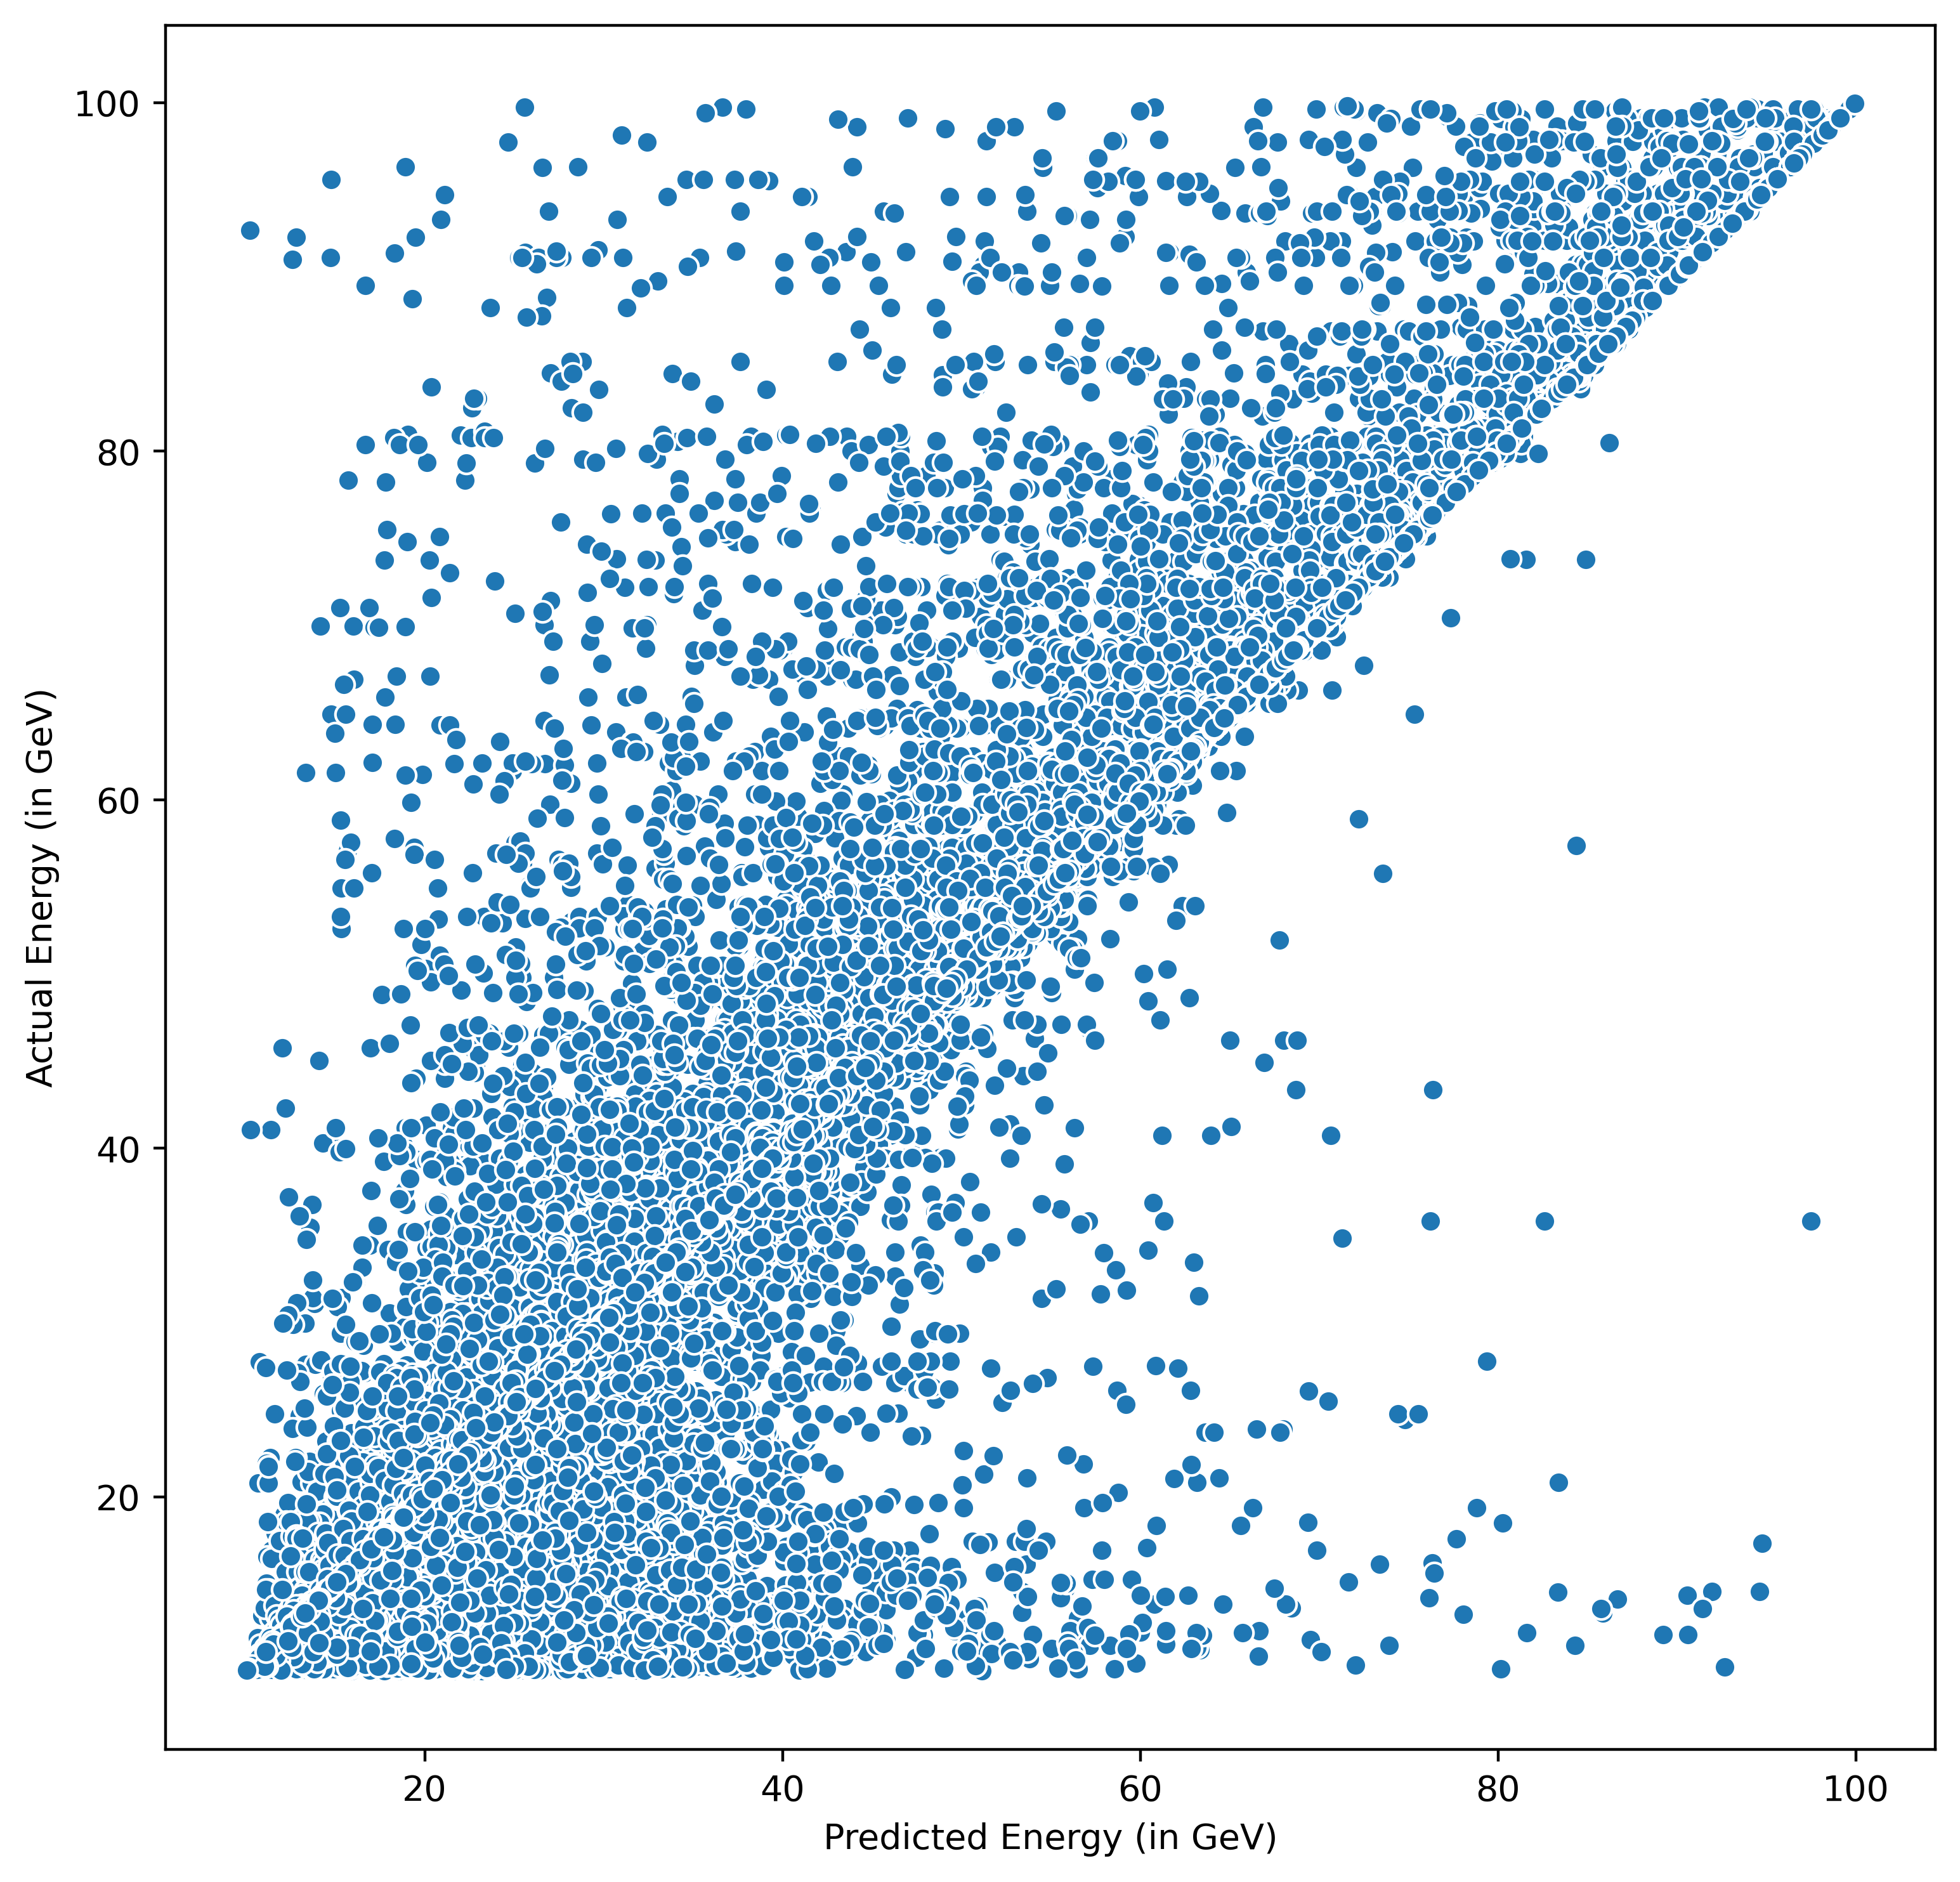
\includegraphics[width=0.44\textwidth, keepaspectratio]{results_rf}\label{fig:test_rf}}
\subfloat[50 Evaluation Timeslices]{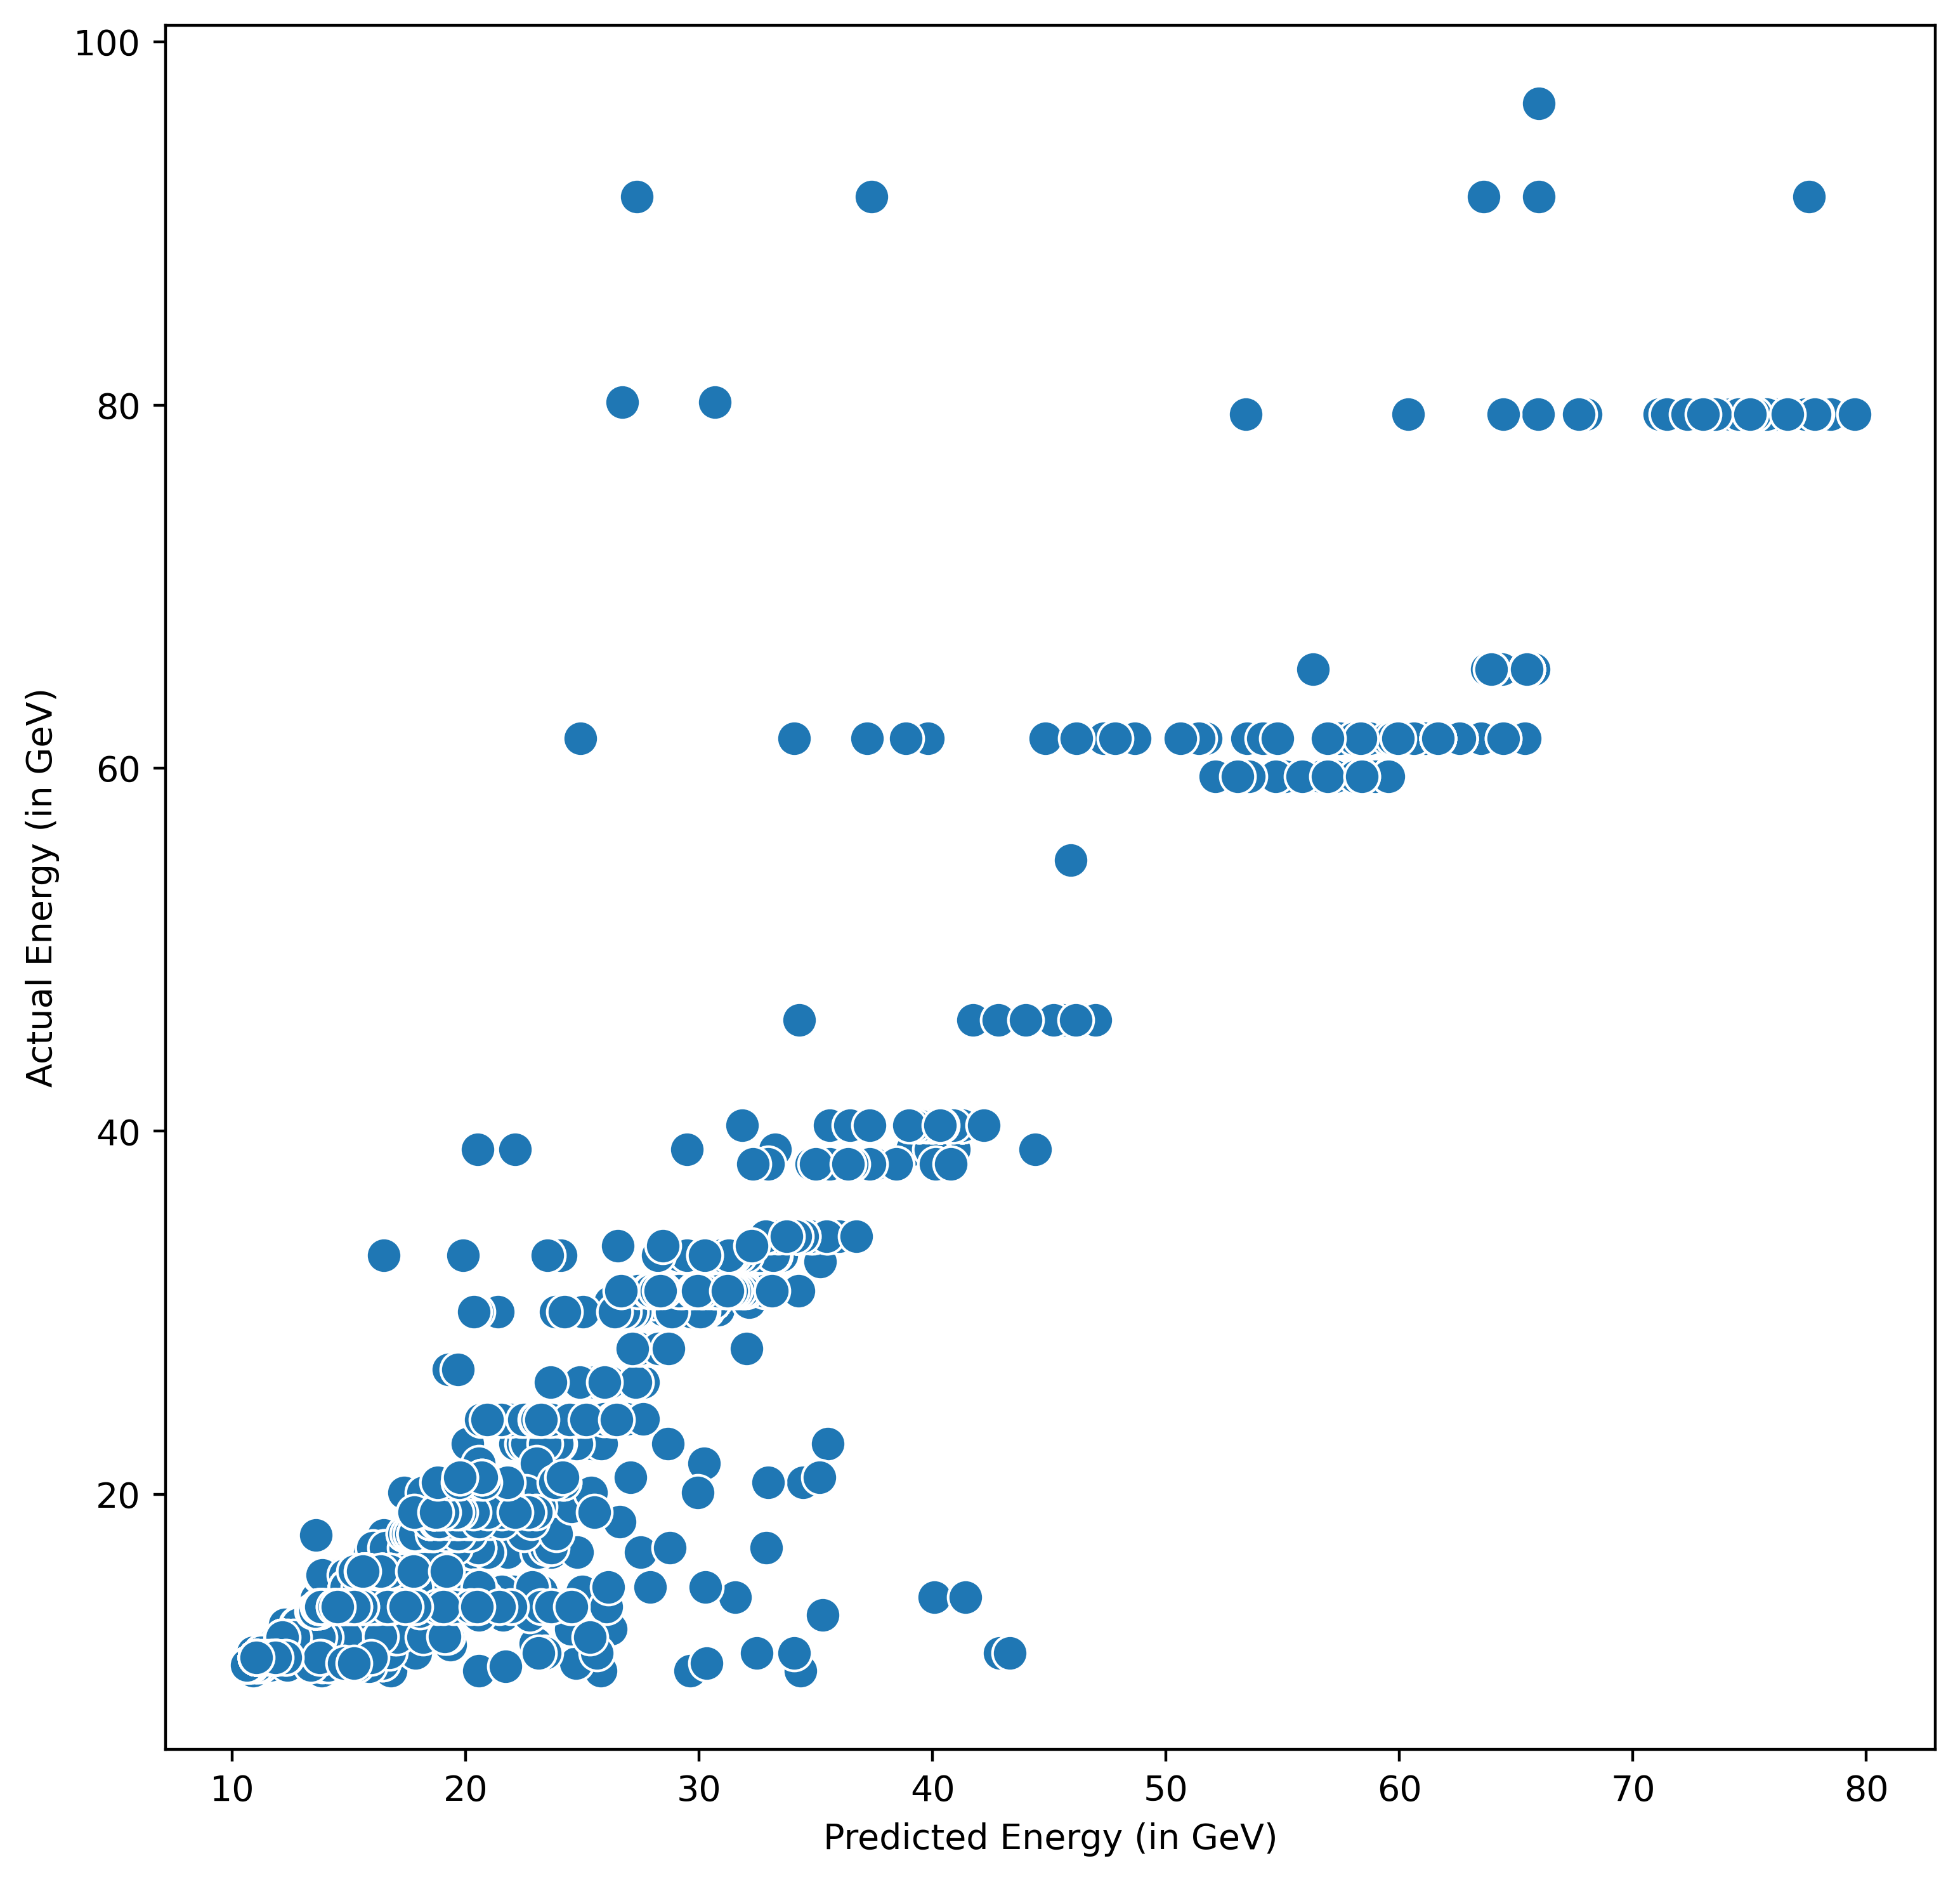
\includegraphics[width=0.44\textwidth, keepaspectratio]{results_eval_rf}\label{fig:eval_rf}}
\caption[]{Random Forest Regressor: Actual vs Predicted Energy Values on Testing and Evaluation Data}
\label{fig:results_rf}
\end{figure}

Figure \ref{fig:results_rf} shows the predicted versus actual energy values on the training and 50 holdout timeslices. The model is much better at predicting across all levels of energy due to the closeness of the points to the diagonal. Sub-figure \ref{fig:test_rf} indicates that the model still predicted some high energy events as lower energy events. 

\subsection{Regression Analysis}
Overall, random forests performed the best out of the applied models. The minimum energy predicted was 12.138 GeV for events containing only 32 hits. This could be attributed to the algorithm itself. They are ensemble algorithms comprising multiple trees \cite{scikit-learn}. The models are diverse since each tree is learnt on a random sample of the data and at each node, a random set of feature are considered \cite{scikit-learn}.  Decision trees are known to overfit and learn the data. This was noted in the experiment due to the difference in R2 values between training and testing (Table \ref{tab:decision_scores}). While the tree was pruned by lowering the maximum depth of the tree, it still showed overfitting. It could be because the problem itself is too hard for the tree to learn and not suited for the Decision tree's learning rules. The algorithm may also require more complex pruning techniques such as weight-based pre-pruning \cite{breiman1984classification, scikit-learn}. In both cases, the model was biased towards predicting high energy events as low energy events. This was atypical to results from other energy inference research \cite{km3net_2017, abbasi2011measurement, d2018flavor} where models were better at predicting higher energy events associated with a larger number of hits. This bias may be due to the splitting parameter set in the experiments. A large value for splitting trees results in a deeper tree with "cleaner" nodes and higher variance, but a lower value limits the splits, leading to higher bias and lower variance \cite{scikit-learn}. 

\section{Summary}
Figures \ref{fig:3D_pipeline} and \ref{fig:4D_pipeline} summarise the two alternate pipeline approaches examined in this chapter. Figure \ref{fig:3D_pipeline} outlines the alternate 3D points-based pipeline. Three permutations of the KM3NeT dataset were obtained and processed using radius-based outlier filter, but no 3D meshes were generated. This pipeline was explored to try and achieve faster processing, but it did not result in suitable learning. Figure \ref{fig:4D_pipeline} outlines the second alternative pipeline. The pipeline employed 4D data, ie., it did not make use of the three dataset permutations. Again, no 3D meshes were generated. This approach too demonstrated the network's inability to classify between the two classes. Finally, energy inference experiments indicated random forests as the best candidate for regression-based approach. Lack of through testing with varied, larger datasets however, indicate more work in the area.

\begin{figure}[ht!]
    \centering
    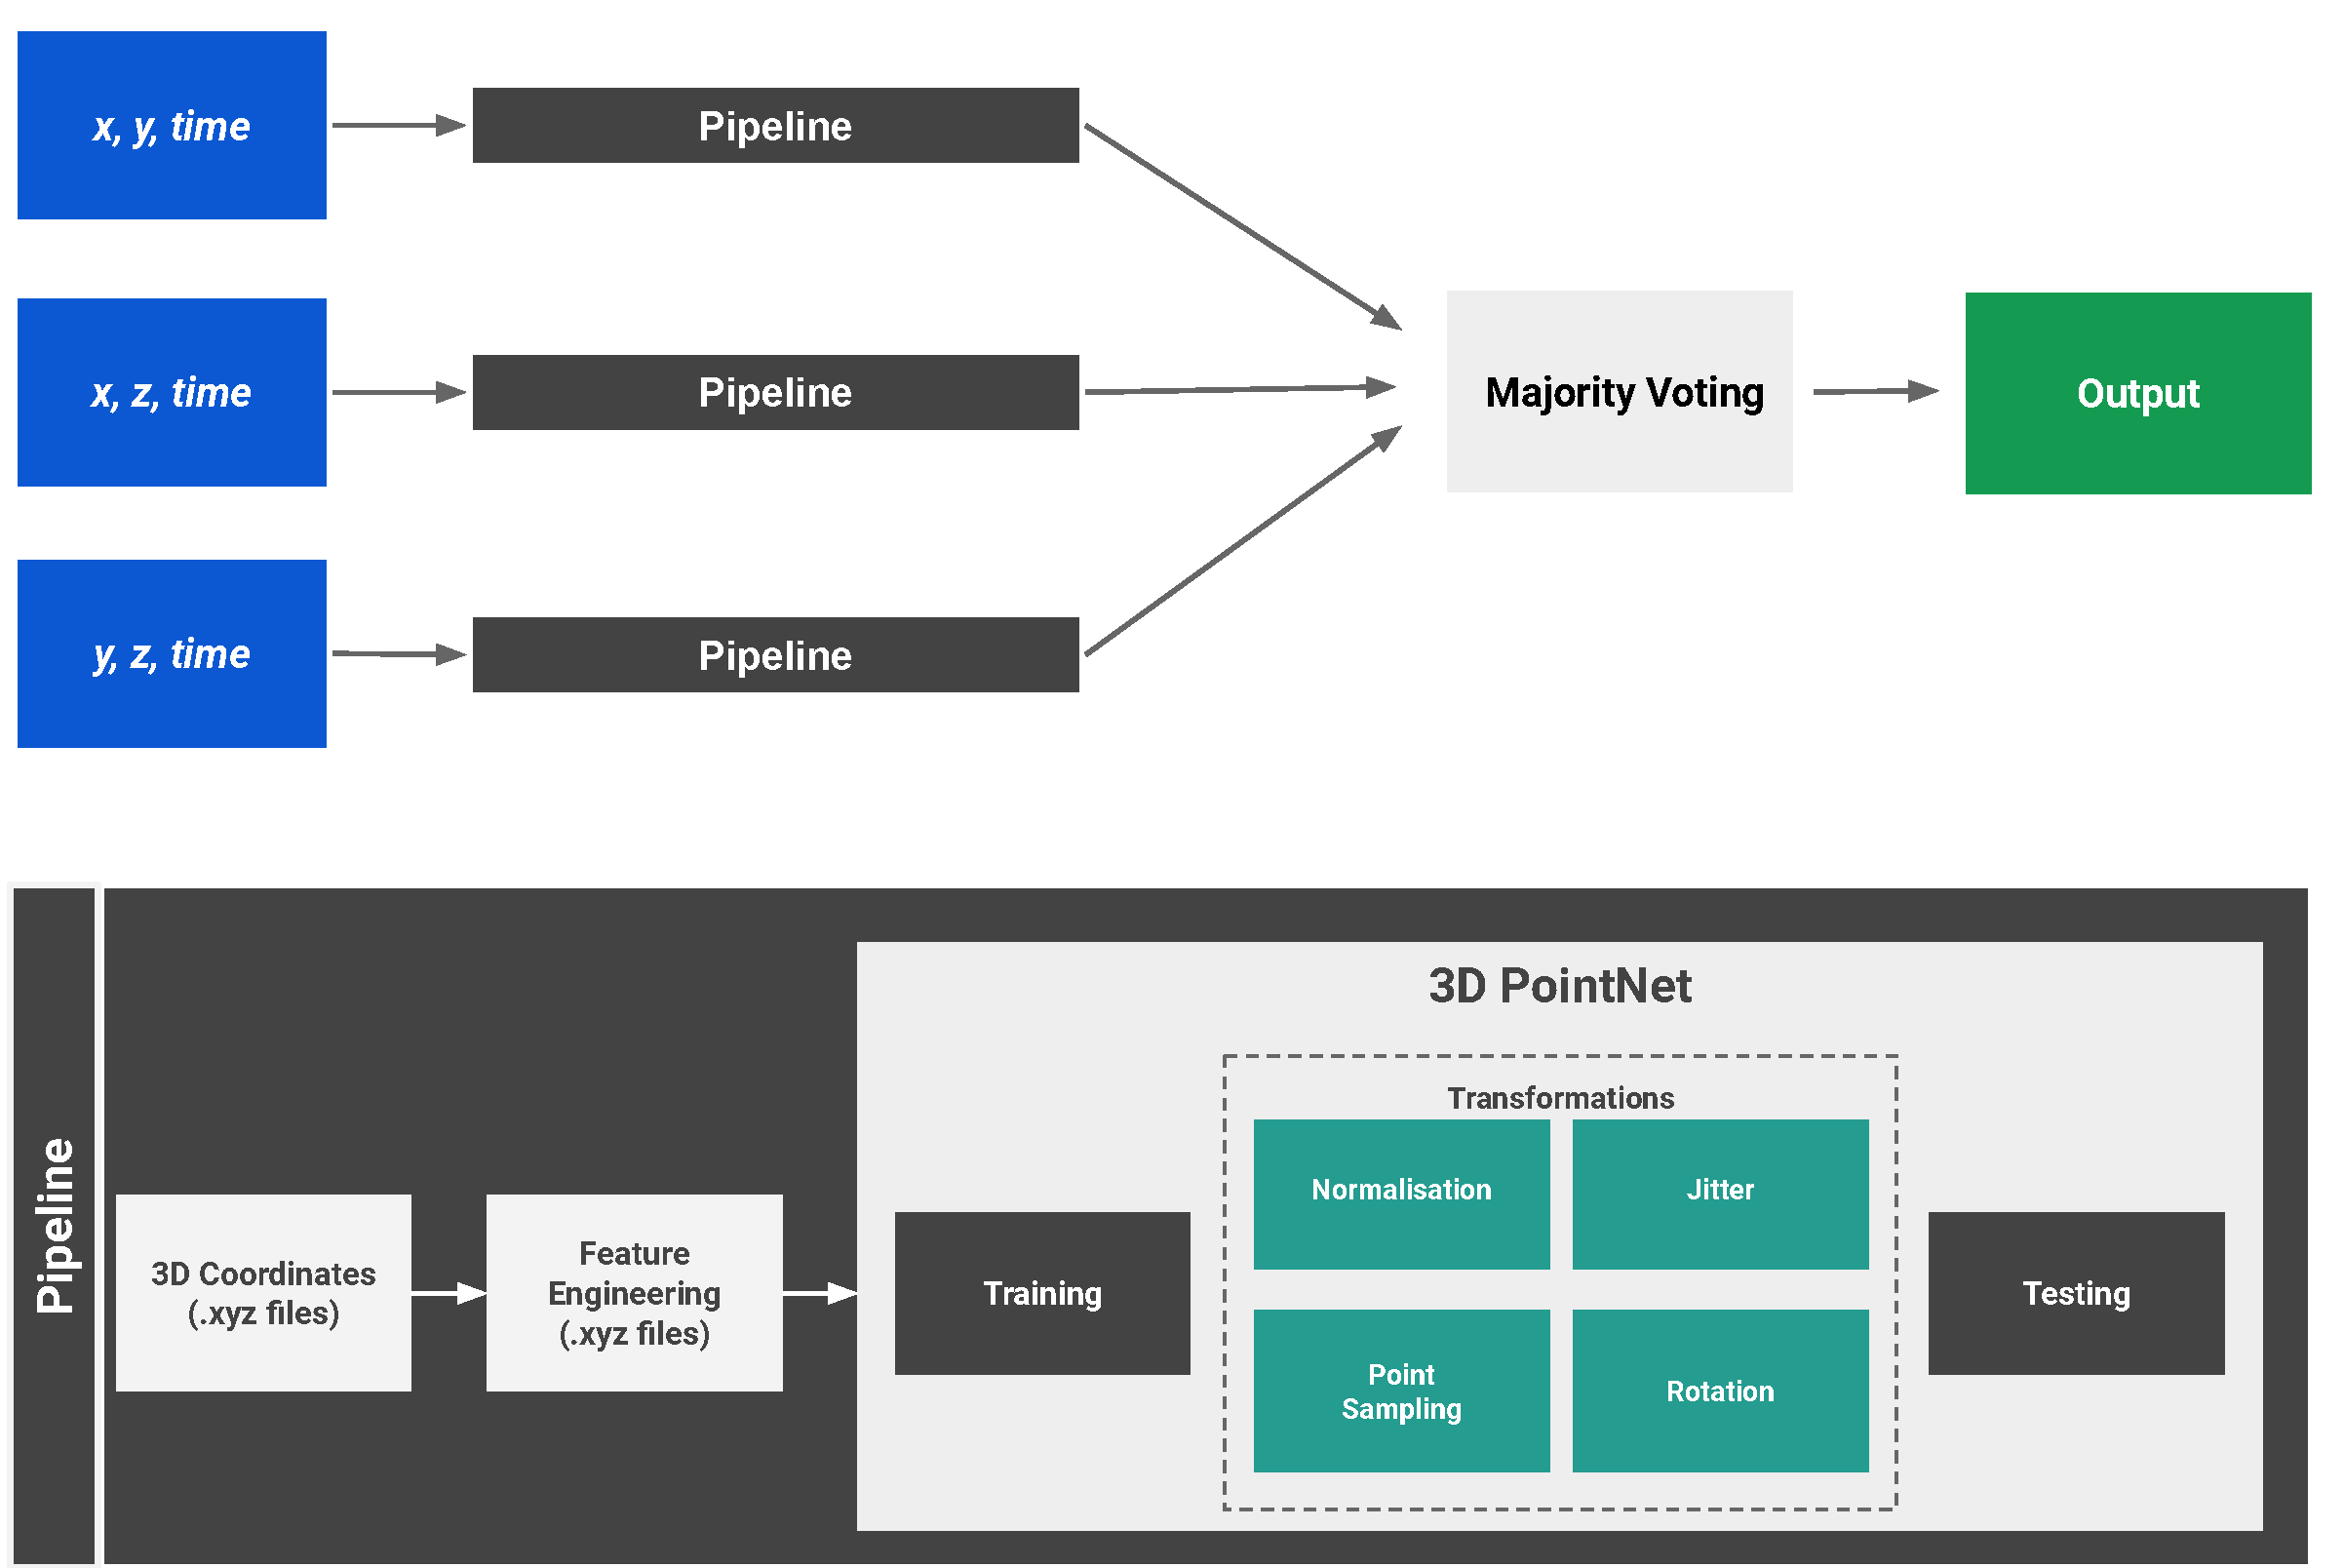
\includegraphics[width=\textwidth,keepaspectratio]{3D_pipeline.pdf}
    \caption{Alternate Pipeline I: 3D Points-based PointNet}
    \label{fig:3D_pipeline}
\end{figure}

\begin{figure}[ht!]
    \centering
    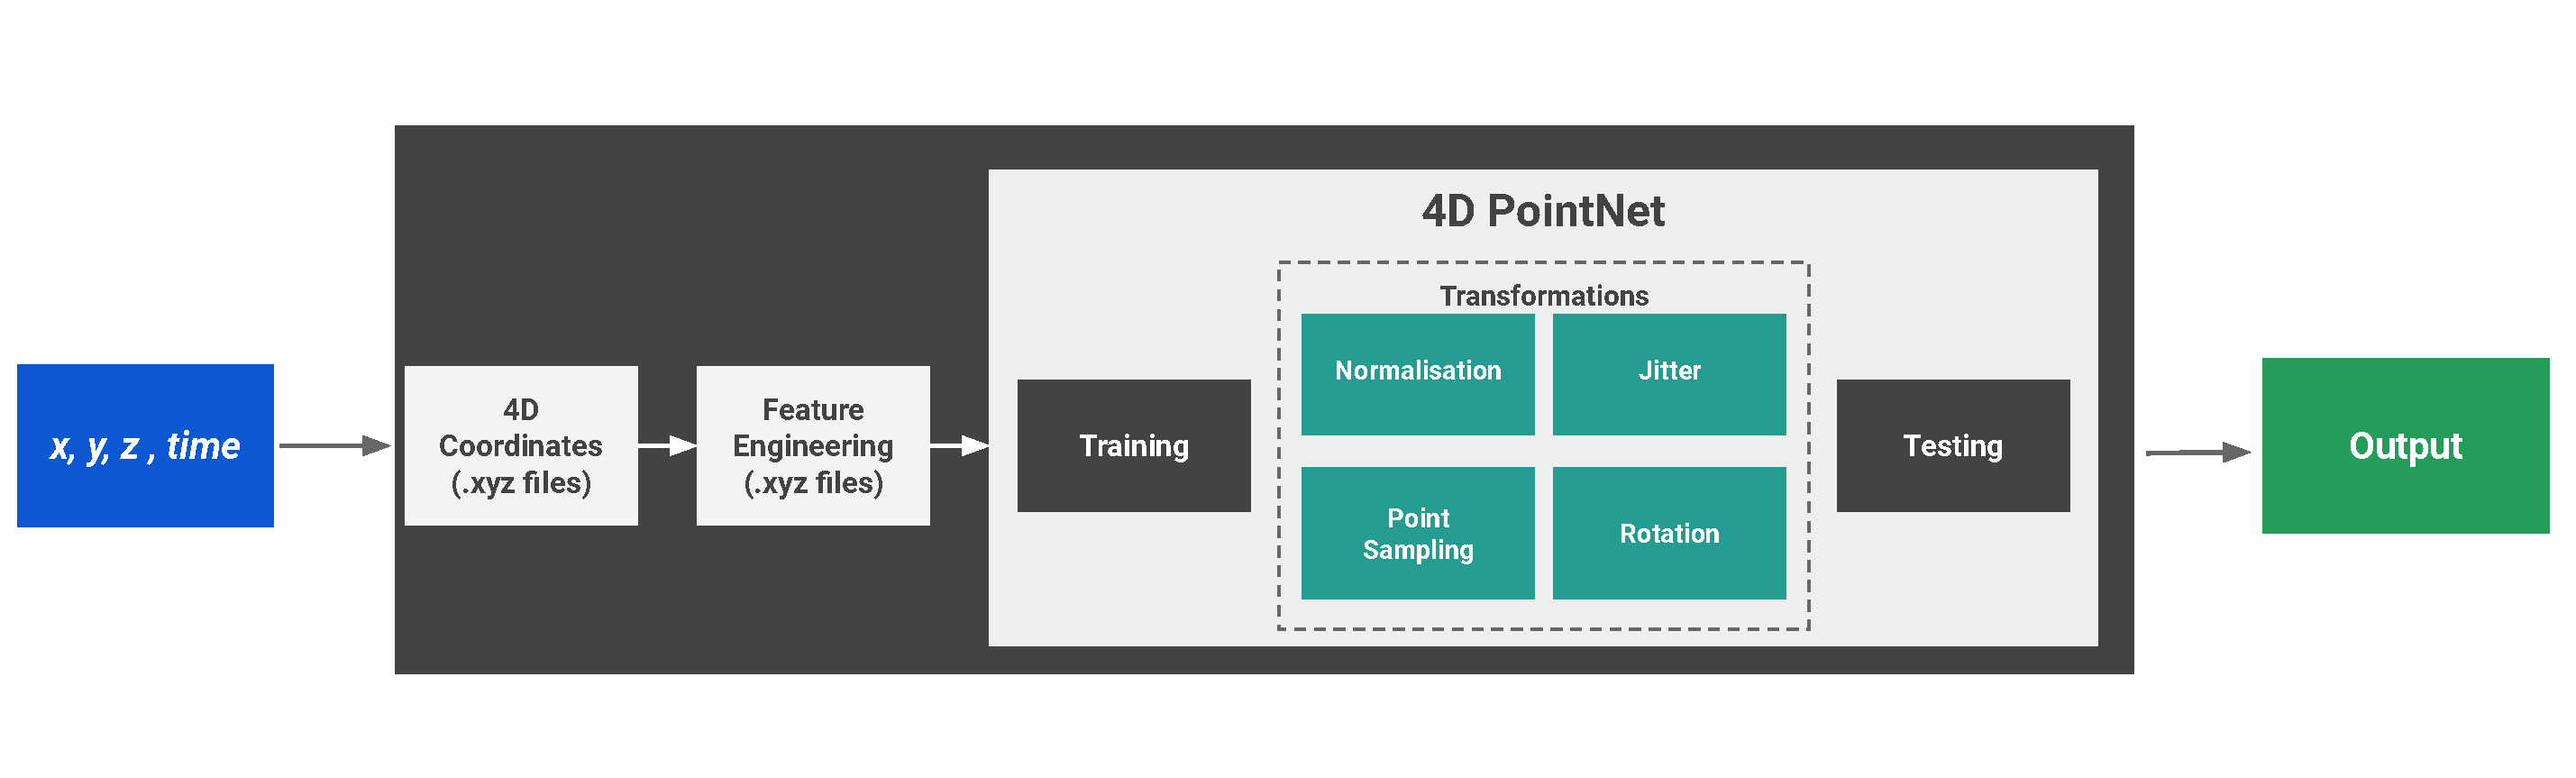
\includegraphics[width=\textwidth,keepaspectratio]{4D_pipeline.pdf}
    \vspace{-1cm}
    \caption{Alternate Pipeline II: 4D PointNet}
    \label{fig:4D_pipeline}
\end{figure}


\let\cleardoublepage\clearpage